\documentclass[10pt,xcolor={dvipsnames}]{beamer}
\usetheme[
%%% option passed to the outer theme
%    progressstyle=fixedCircCnt,   % fixedCircCnt, movingCircCnt (moving is deault)
  ]{Feather}
  
% If you want to change the colors of the various elements in the theme, edit and uncomment the following lines

% Change the bar colors:
\setbeamercolor{Feather}{fg=NavyBlue!20,bg=NavyBlue}

% Change the color of the structural elements:
\setbeamercolor{structure}{fg=NavyBlue}

% Change the frame title text color:
\setbeamercolor{frametitle}{fg=black!5}

% Change the normal text colors:
\setbeamercolor{normal text}{fg=black!75,bg=gray!5}

%% Change the block title colors
\setbeamercolor{block title}{use=Feather,bg=Feather.fg, fg=black!90} 


% Change the logo in the upper right circle:
%\renewcommand{\logofile}{example-grid-100x100pt} 
%% This is an image that comes with the LaTeX installation
% Adjust scale of the logo w.r.t. the circle; default is 0.875
% \renewcommand{\logoscale}{0.55}

% Change the background image on the title and final page.
% It stretches to fill the entire frame!
% \renewcommand{\backgroundfile}{example-grid-100x100pt}

%-------------------------------------------------------
% INCLUDE PACKAGES
%-------------------------------------------------------

\usepackage[utf8]{inputenc}
\usepackage[english]{babel}
\usepackage[T1]{fontenc}
\usepackage{amsfonts}
% \usepackage{helvet}

%% Load different font packages to use different fonts
%% e.g. using Linux Libertine, Linux Biolinum and Inconsolata
 %\usepackage{libertine}
% \usepackage{zi4}

%% e.g. using Carlito and Caladea
%\usepackage{carlito}
%\usepackage{caladea}
\usepackage{amssymb, amsmath, amsthm}
\usepackage{zi4}
\graphicspath{ {figures/}{figures/eps/}{figures/pdf/} }% specify the path where figures are located
\usepackage{amsmath}
\usepackage{amscd,latexsym,amsfonts,amstext,amsbsy}
\usepackage[mathscr]{euscript} %for european script
\usepackage{colortbl}
\usepackage{graphics}
\usepackage{graphicx}
\usepackage{epstopdf}
\usepackage{amssymb}
\usepackage{amsmath}
\usepackage{cite}
\usepackage{color,soul}
\usepackage{array}
\usepackage{xcolor}
\newcolumntype{C}[1]{>{\centering\let\newline\\\arraybackslash\hspace{0pt}}m{#1}}
\usepackage[config, labelfont={bf}]{caption,subfig}
\usepackage{float}
\usepackage{caption}
\usepackage{comment}
\newcolumntype{K}[1]{>{\centering\arraybackslash}p{#1}}



%% e.g. using Venturis ADF Serif and Sans
% \usepackage{venturis}

%-------------------------------------------------------
% DEFFINING AND REDEFINING COMMANDS
%-------------------------------------------------------

% colored hyperlinks
\newcommand{\chref}[2]{
  \href{#1}{{\usebeamercolor[bg]{Feather}#2}}
}



\AtBeginSection[]
{
  \begin{frame}<beamer>
    \frametitle{Overview}
    \tableofcontents[currentsection]
  \end{frame}
}



\newenvironment<>{varblock}[2][\textwidth]{%
  \setlength{\textwidth}{#1}
  \begin{actionenv}#3%
    \def\insertblocktitle{#2}%
    \par%
    \usebeamertemplate{block begin}}
  {\par%
    \usebeamertemplate{block end}%
  \end{actionenv}}


  
  
  
\begin{document}
\newcommand{\cfbox}[2]{%
    \colorlet{currentcolor}{.}%
    {\color{#1}%
    \fbox{\color{currentcolor}#2}}%
}




\title[] % [] is optional - is placed on the bottom of the sidebar on every slide
{ % is placed on the title page
      {\textbf{Two Models: Heroin Epidemic and Harvesting Forest Products}}
}

\subtitle[Oral Exam]
{
      
}

\author[T. Phillips]
{    \large{Tricia Phillips} \\ 
\vspace{0.5cm}
Advised by: Dr. Suzanne Lenhart and \\ Dr. Christopher Strickland
      %{\ttfamily lilqna.v@gmail.com}\\[1em]
      %with v1.1 modifications by LianTze Lim (Overleaf)
}


%\institute{Dissertation Defense}
%{%
   %   Faculty of Mathematics, Informatics and Information Technologies\\
     % Plovdiv University ``Paisii Hilendarski''
%}

%\date{\today}
\date{May 25, 2018}


%\title[Optimal Control of Vacc for \textit{C. diff}]{Optimal Control of Vaccination Rate in an Epidemiological Model of \textit{Clostridium difficile} Transmission} 
%\author[Stephenson]{Brittany Stephenson \\
 %Cristina Lanzas\\
%Suzanne Lenhart\\
%Judy Day}
%\institute[UTK]{ University of Tennessee, Knoxville\\ }
%\date{\today}
  
 



{\1% % this is the name of the PDF file for the background
\begin{frame}[plain,noframenumbering] % the plain option removes the header from the title page, noframenumbering removes the numbering of this frame only
  \titlepage % call the title page information from above
\end{frame}}
  
  
\begin{frame}{Content}{}
\frametitle{Overview}
\tableofcontents
\end{frame}
  
  
\section{Motivation for Heroin Model}



\begin{frame}
\frametitle{Motivation}
{\color{beamer@headercolor}  \textbf{Opioids}} 

\begin{itemize}

\item<1> American Pain Society aggressively pushed idea of
pain as the fifth vital sign in mid 1990's as they believed pain was being undertreated in doctor offices and hospitals. 
\item <1> In 2000, Joint Commission required physicians to accept and
respect the self-reporting of pain by patients. 
\item <1> Early 2000s, drug manufacturers funded publications and physicians to support opioid use for pain control. 
\item<1> Number of opioid prescriptions that pharmacies distributed in 2011 was almost triple that of 1991.
\end{itemize}


\end{frame}


\begin{frame}
\frametitle{Motivation}
\begin{itemize}

\item<1> The misuse of opioids, a drug class including prescription pain relievers and heroin, is rampant in today's society.
\item<1> The opioid crisis was declared a public health emergency in October 2017 by the United States Department of Health and Human Sciences.
\item<1> Treatments available for opioid and heroin use; involves medications (methadone, naltrexone, etc.), counseling, behavioral therapies. 
\end{itemize}


\end{frame}




\begin{frame}
\frametitle{Motivation}
 \vspace{-1cm}

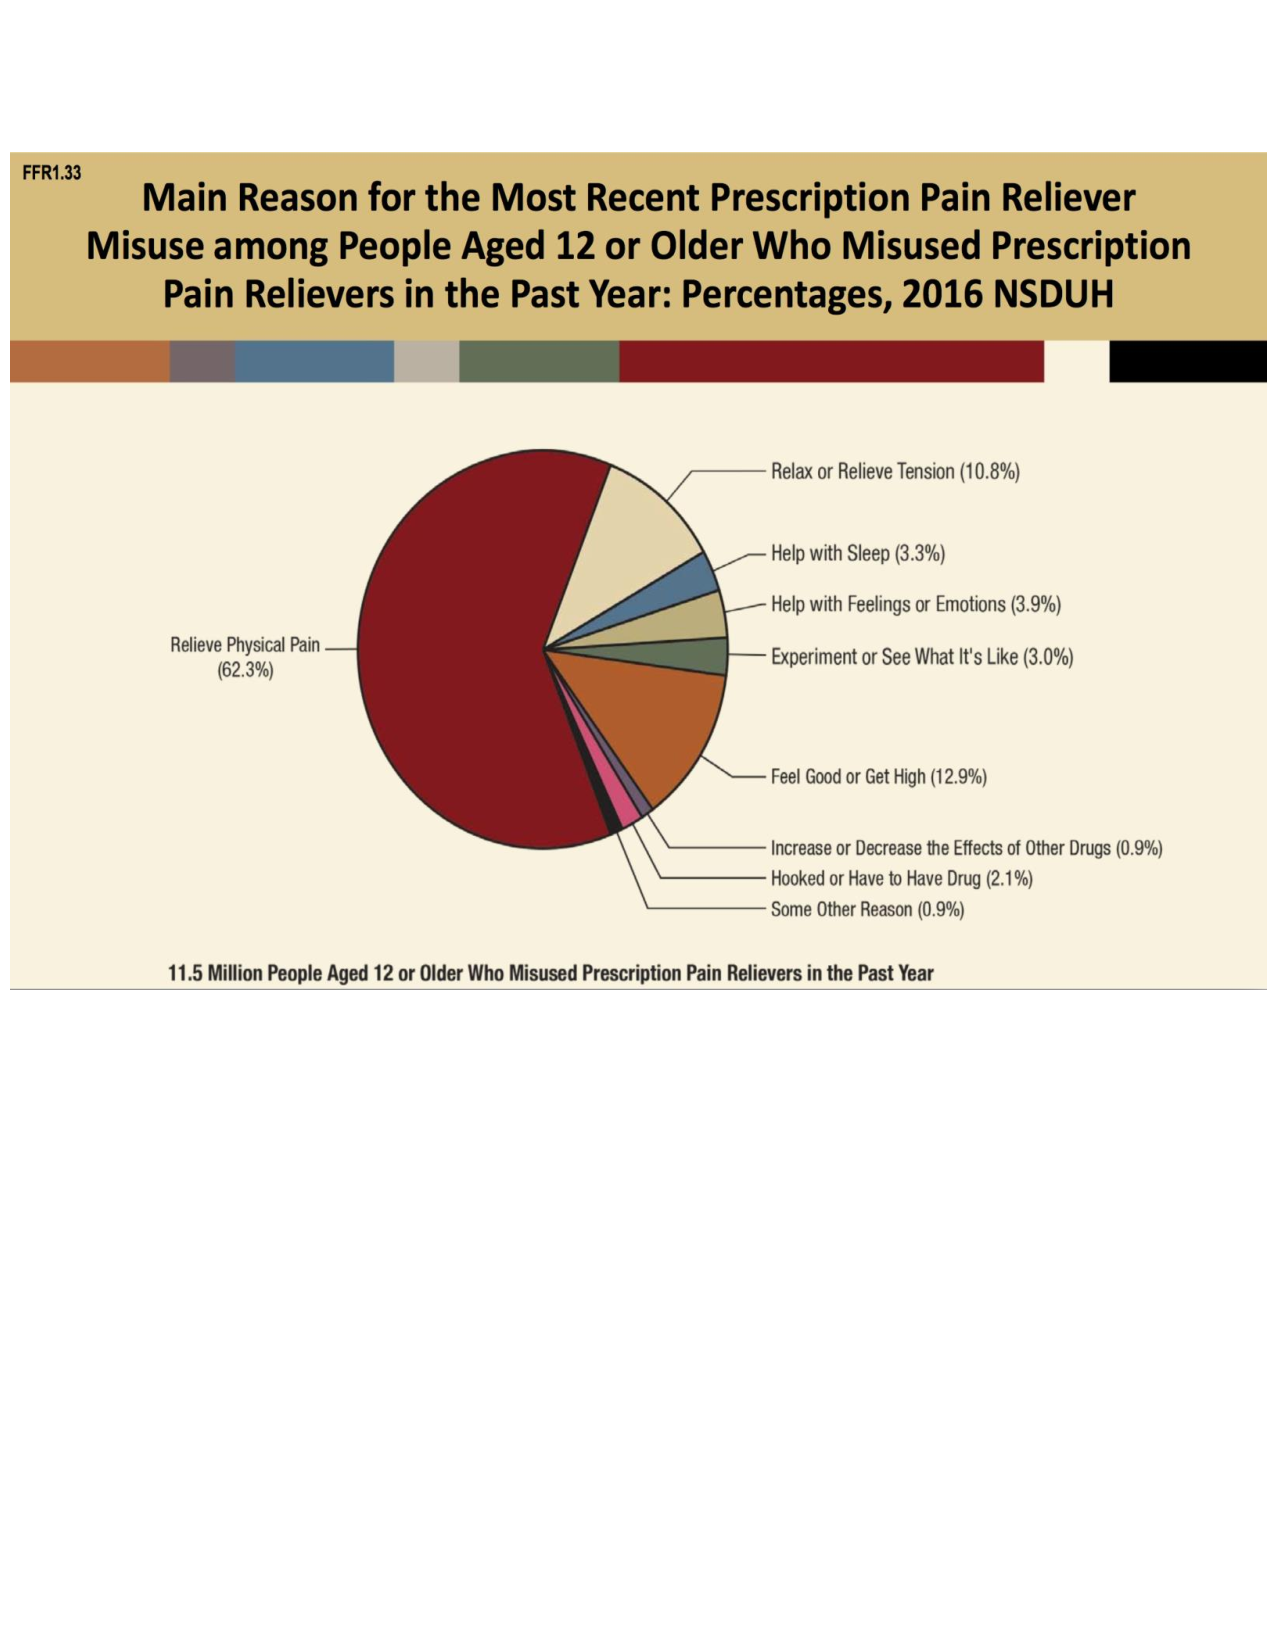
\includegraphics[height=12cm, width=11cm]{reason_pain_relievers.pdf}
\vspace{-5cm}

\begin{center}
\textbf{Source:} 2016 National Survey on Drug Use and Health 
\end{center}
\end{frame} 


\begin{frame}
\frametitle{Motivation}
 \vspace{-1cm}
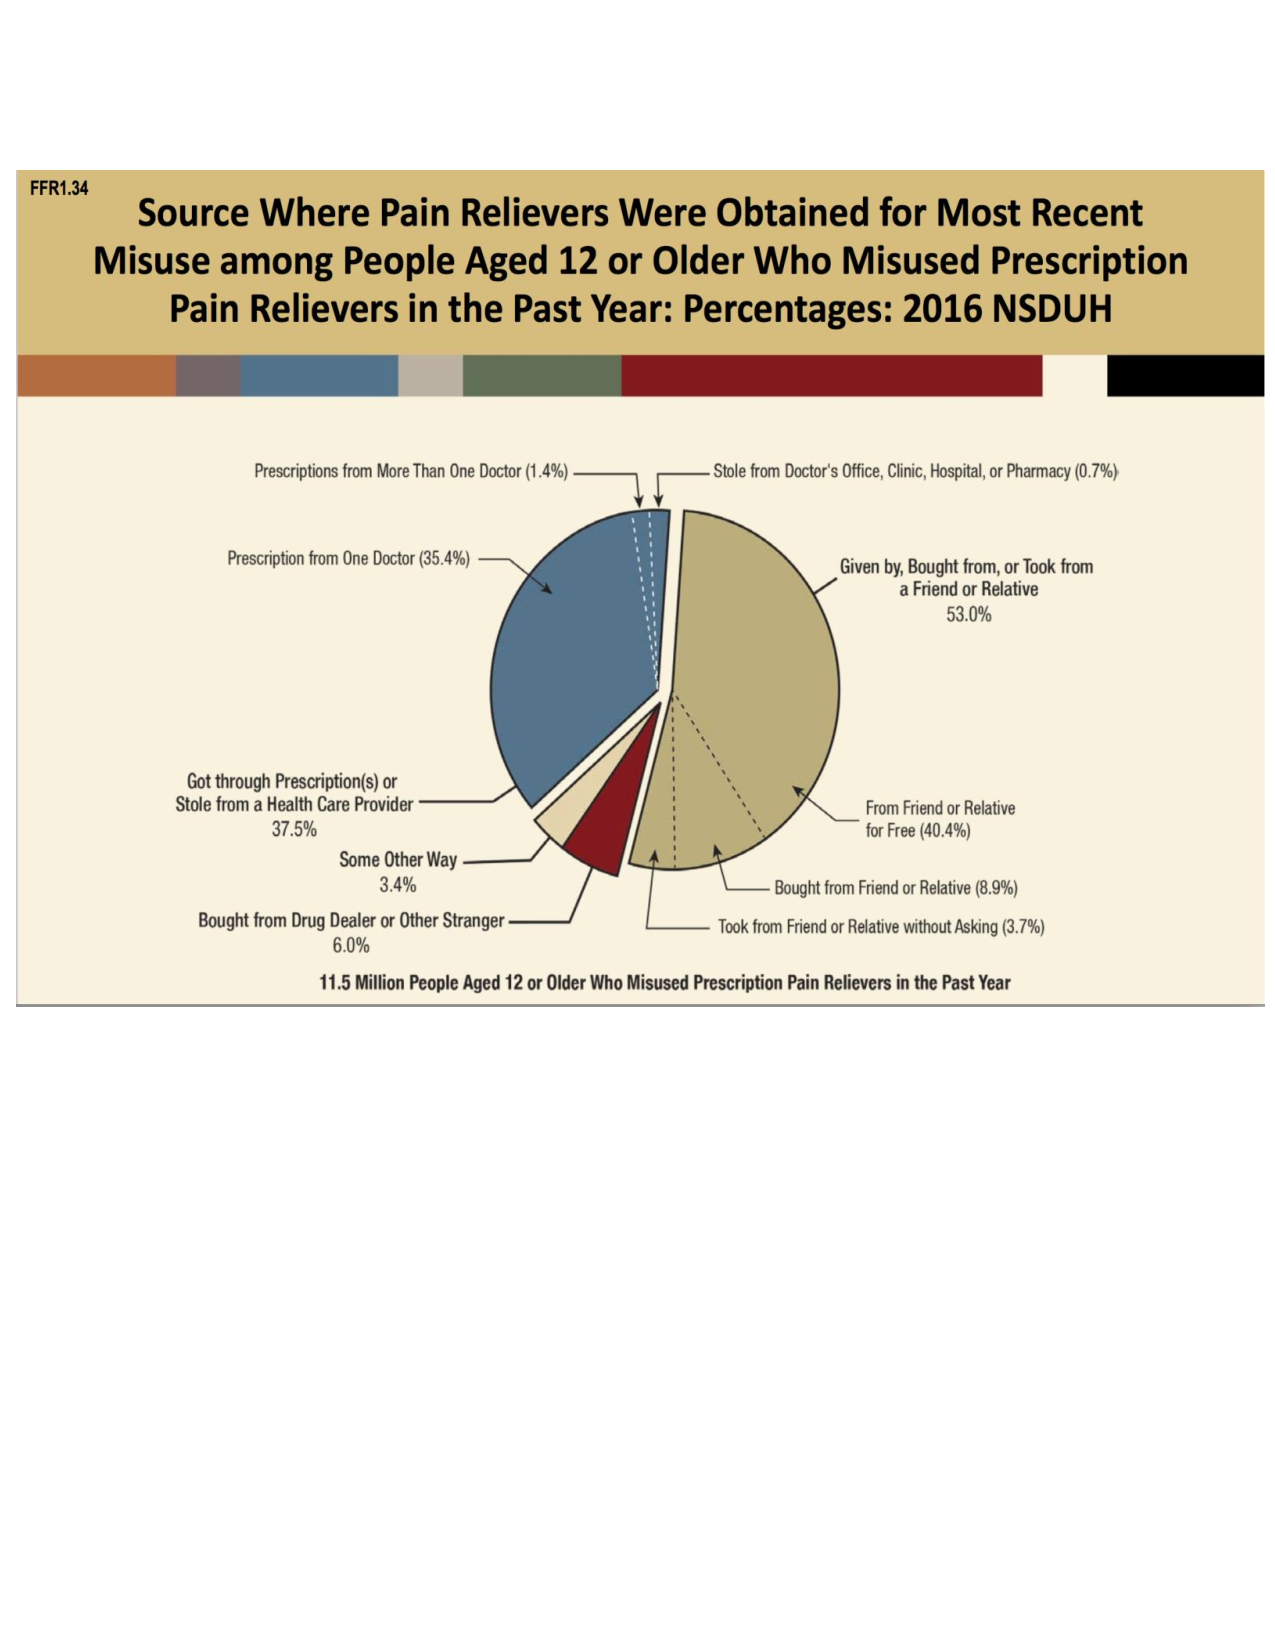
\includegraphics[height=12cm, width=11cm]{source_pain_relievers.pdf}
\vspace{-5cm}

\begin{center}
\textbf{Source:} 2016 National Survey on Drug Use and Health 
\end{center}

\end{frame} 


\begin{frame}
\frametitle{Motivation}


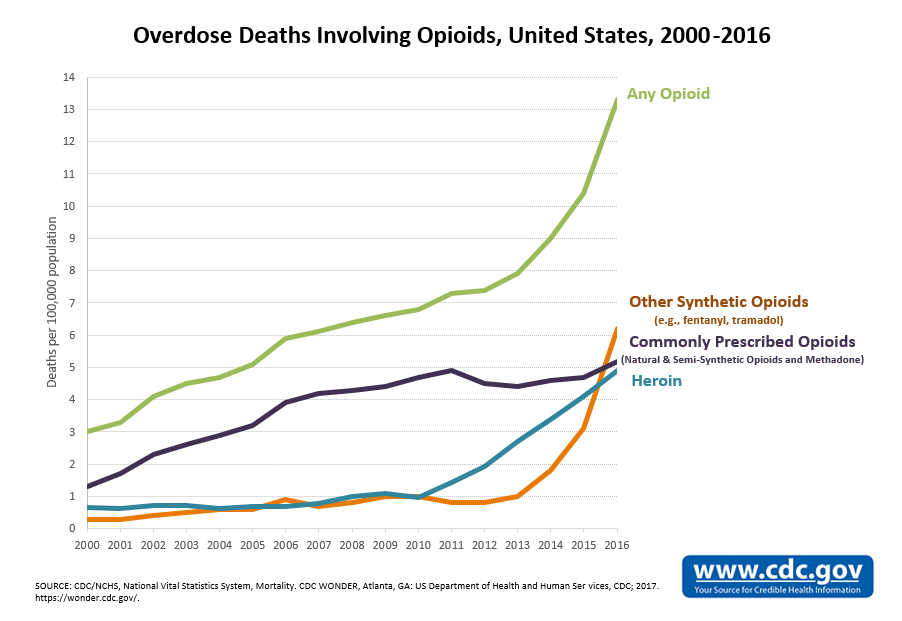
\includegraphics[height=6cm, width=11cm]{opioid_overdoses.png}


\begin{center}
\textbf{Source:} Centers for Disease Control and Prevention 
\end{center}
\end{frame} 



\begin{frame}
\frametitle{Motivation}

{\color{beamer@headercolor}  \textbf{Heroin}}
\begin{itemize}

\item<1> Dramatic increase in accessibility to heroin and the lower cost of the drug has influenced prescription opioid users to turn to heroin.
\item<1> Based on 2002-2012 NSDUH data, study found heroin initiation 19 times more likely for non-medical opioid users than non-users. 
\item<1> Estimated 80\% of heroin users at the national level used prescription opioids previously. 
\item<1> Heroin overdose deaths have increased significantly in recent years. 
\item<1> In 1960s, heroin users composed mainly of young, non-white men in urban areas with initial opioid being heroin; present day, shifted to older, white, rural/suburban, men and women. 
\end{itemize}


\end{frame}



\begin{frame}
\frametitle{Motivation}
\vspace{-1cm}
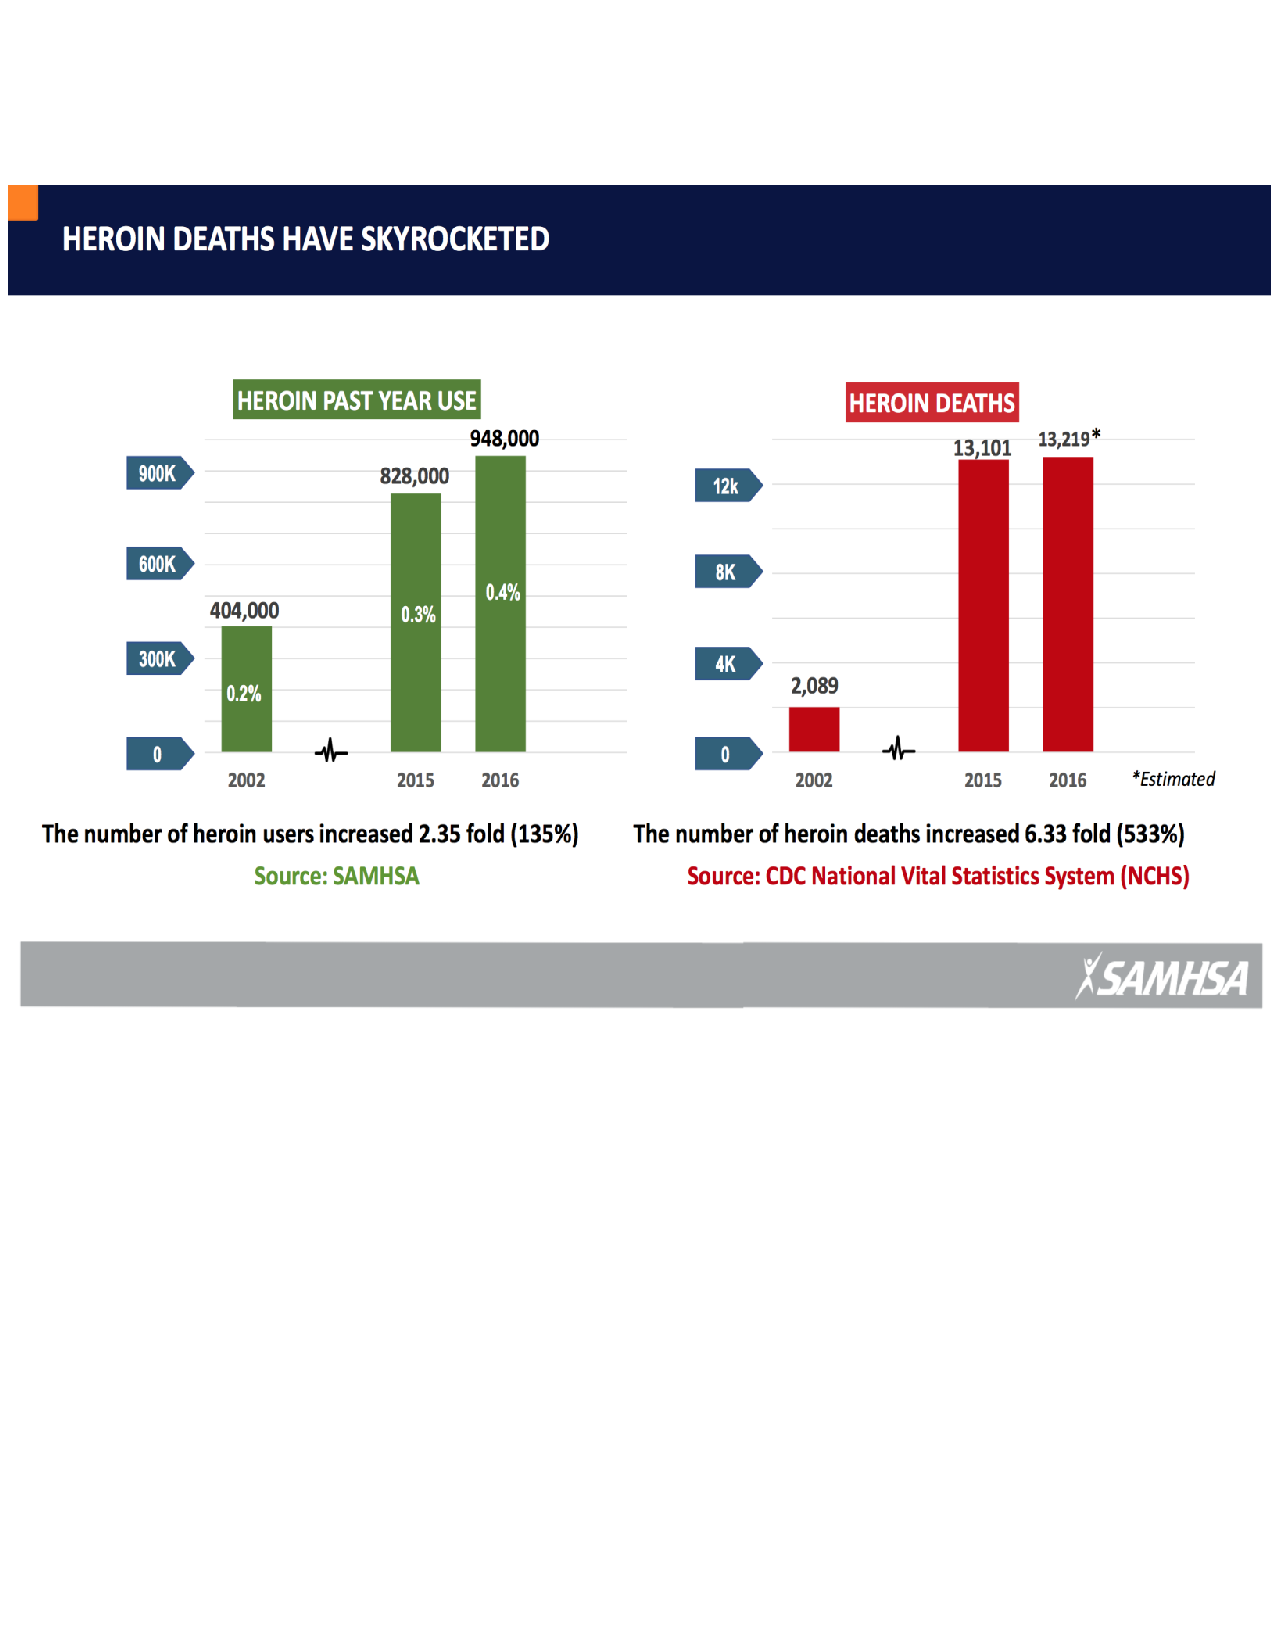
\includegraphics[height=12cm, width=11cm]{heroin_deaths.pdf}
 \vspace{-5cm}

\begin{center}
\textbf{Source:}  2016 National Survey on Drug Use and Health Report from SAMSHA.gov
\end{center}
\end{frame} 






\begin{frame}
\frametitle{Challenges}


\begin{itemize}
\item<1> Fentanyl is a surgical-grade synthetic opioid up to 50 times more potent than heroin. 
\item<1> Fentanyl is mixed with heroin to increase effect; unknown purity increases overdose risk. 
\item<1> Difficulty in modeling due to variability of the purity of heroin. 
\item<1> 1 in every 5 overdose deaths have multiple drugs present, difficult to determine actual cause of death. 
\item<1> Opioid misuse, abuse, dependency, addiction and use disorder often not clearly defined in literature/difficult to know exactly what is intended. 
\end{itemize}


\end{frame}



\begin{frame}
\frametitle{Motivation}
\vspace{-1cm}
 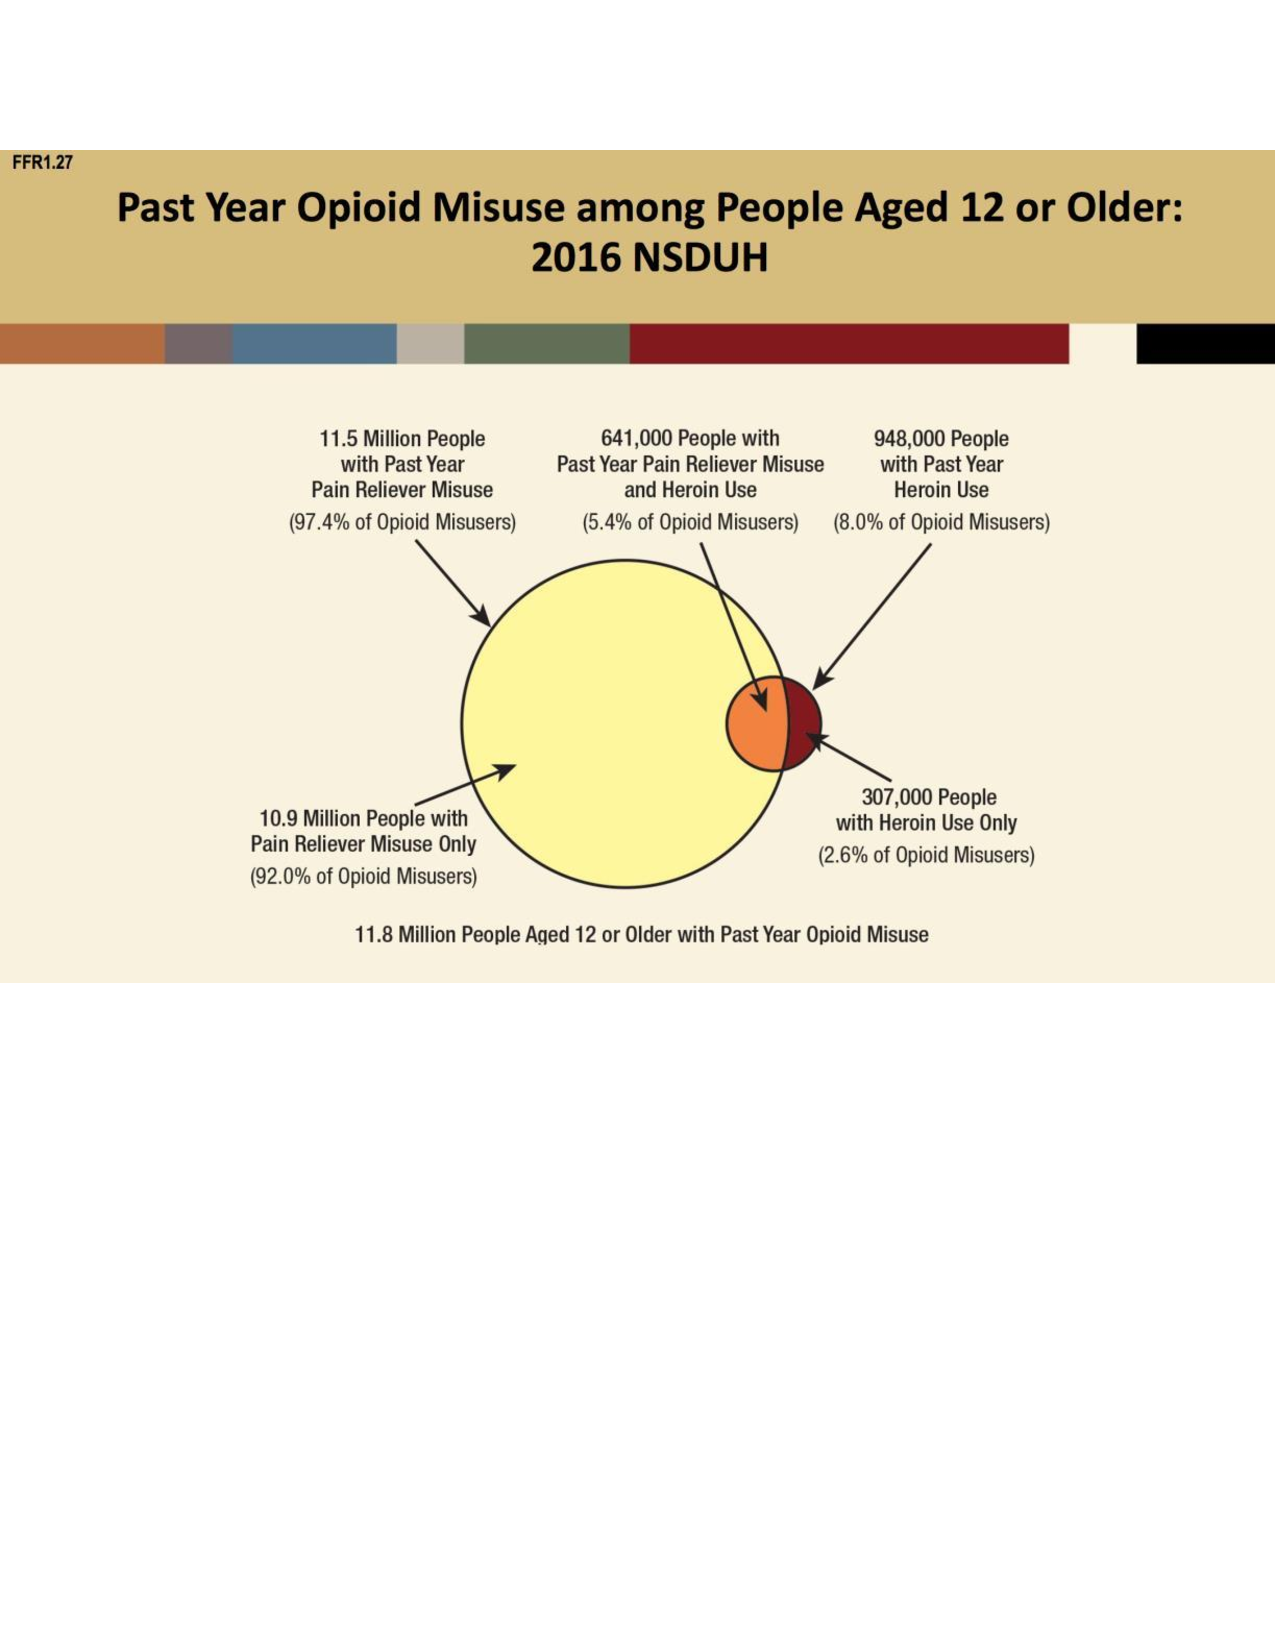
\includegraphics[height=12cm, width=11cm]{past_year_opioid_misuse.pdf}
 \vspace{-5cm}

\begin{center}
\textbf{Source:} 2016 National Survey on Drug Use and Health Report
\end{center}

\end{frame}





\begin{frame}
\frametitle{Previous Work}
\begin{itemize}

\item[]<1> {\color{beamer@headercolor} Opioid Model} 
\begin{itemize}
\item[-]<1> Dr. Christopher Strickland and collaborators, Nicholas Battista and Leigh Pearcy, developed a population-level model for the opioid epidemic (excluding heroin) using a system of ODE's.
\end{itemize} 
\vspace{0.4cm}
\item[]<1> {\color{beamer@headercolor} Population Classes } 
\begin{itemize}
\item[-]<1> Susceptibles ($S$): not taking prescription opioids, nor recovering from opioid addiction. \\
\item[-]<1> Prescription opioid users ($P$): opioid-prescribed individuals not considered addicted. 
\item[-]<1>  Opioid addicts ($A$): addicted to opioids. 
\item[-]<1> Individuals in treatment/rehabilitation ($R$): undergoing treatment for their addiction to opioids. 
\end{itemize}
\end{itemize}
\end{frame}




\begin{frame}
\frametitle{Previous Work}
\includegraphics[height=6cm, width=10.5cm]{Opioid_schematic.pdf} \\
%\begin{itemize}[-]
\begin{center}
Schematic diagram for opioid-only model 
\end{center}
%\end{itemize}
\end{frame}






\begin{frame}
\frametitle{Previous Work}

\small
$$\dfrac{dS}{dt} = -\alpha S - \beta (1- \xi) SA  -\beta \xi SP +\epsilon P +\delta R + 
\mu (P+R) + \mu^{*}A \hspace{1cm} $$ 


\vspace{.1cm}

$$\dfrac{dP}{dt} = \alpha S - \epsilon P  - \gamma P - \mu P \hspace{1cm}$$

\vspace{.1cm}

$$\dfrac{dA}{dt} = \gamma P + \sigma R +\beta (1- \xi) SA  +\beta \xi SP +\nu RA -\zeta A -\mu^*A $$ \\

\vspace{.1cm}

$$\dfrac{dR}{dt} = \zeta A -\nu RA -\delta R -\sigma R -\mu R$$



\end{frame}



\begin{frame}
\frametitle{Previous Work}
\begin{itemize}

\item[]<1> {\color{beamer@headercolor} Main Results} 
\begin{itemize}
\item[-]<1> In order to have an addiction-free equilibrium, both addictions that come from prescriptions and addictions from accessibility to excess drugs must be eliminated ($\gamma=0=\xi$).  
\item[-]<1> Near addiction-free state: prevention of prescription opioid users becoming addicted is more important than reducing prescriptions getting into the hands of non-prescribed users to combat the epidemic. 
\item[-]<1> More realistically, outside of addiction-free state: reducing prescription-user addictions, decreasing prescriptions dispensed and increasing entry into treatment are most important to reduce number of addicted. 

\end{itemize}
\end{itemize}
\end{frame}





\section{Heroin Model Formulation}  
  
 \begin{frame}
\frametitle{Model Formulation}
\begin{itemize}
\item {\color{beamer@headercolor}  \textbf{Goals}}: 
\vspace{0.3cm}
\begin{enumerate}[-]
\item Investigate the dynamics behind the opioid and heroin epidemic and identify important conditions relating to the reduction of opioid and heroin addicted individuals. 
\vspace{.2cm}
\item Develop a system of ODEs model consisting of classes of individuals taking prescription opioids, addicted to opioids, using heroin and recovering from opioid addiction, including heroin, and analyze it. 
\vspace{.2cm}
\item Investigate management strategies for how to best treat pain with prescriptions while reducing opioid addiction and heroin use. 
\end{enumerate}
\end{itemize}

\end{frame}
  
  
  
  
  
   \begin{frame}
\frametitle{Model Formulation}

\begin{itemize}
\item[-]<1> We formulated a five class compartmental population model. 

\item[-]<1> {\color{beamer@headercolor} Population Classes} 
\begin{itemize}
\item[-]<1> Susceptibles ($S$): not taking prescription opioids, nor using heroin. \\
\item[-]<1> Prescription opioid users ($P$): opioid-prescribed individuals not considered addicted. 
\item[-]<1>  Opioid addicts ($A$): addicted to opioids. 
\item[-]<1> Heroin users ($H$): addicted to heroin. 
\item[-]<1> Individuals in treatment/rehabilitation ($R$): undergoing treatment for their addiction to opioids or heroin. 

\end{itemize}
\end{itemize}

\end{frame}




\begin{frame}
\frametitle{Model Formulation}
\begin{itemize}
\item[]<1> {\color{beamer@headercolor} Assumptions} 
\vspace{.2cm}
\begin{itemize}
\item[-]<1> Constant population so total death rate is equal to the incoming rates for the susceptible class.  
\vspace{.2cm}
%\item[-]<1> Initial population values are fractions of the entire population. Current initial conditions at the national level: $S_{0}=0.6068$, $P_{0}=0.38$, $A_{0}=0.0062$, $H_{0}=0.0026$, and $R_{0}=0.0044.$
\item[-]<1> Only considering individuals who are addicted to opioids (not just any type of misuse).%; addiction defined as individuals with a pattern of continued non-medical use with the potential for harm. 
\vspace{.2cm}
\item[-]<1> Assume there is no permanent recovery class or immunity to addiction, so recovered individuals go back to the susceptible class. 
\end{itemize}
\end{itemize}
\end{frame}


\begin{frame}
\frametitle{}
\vspace{-.52cm}
\hspace*{-1.08cm} 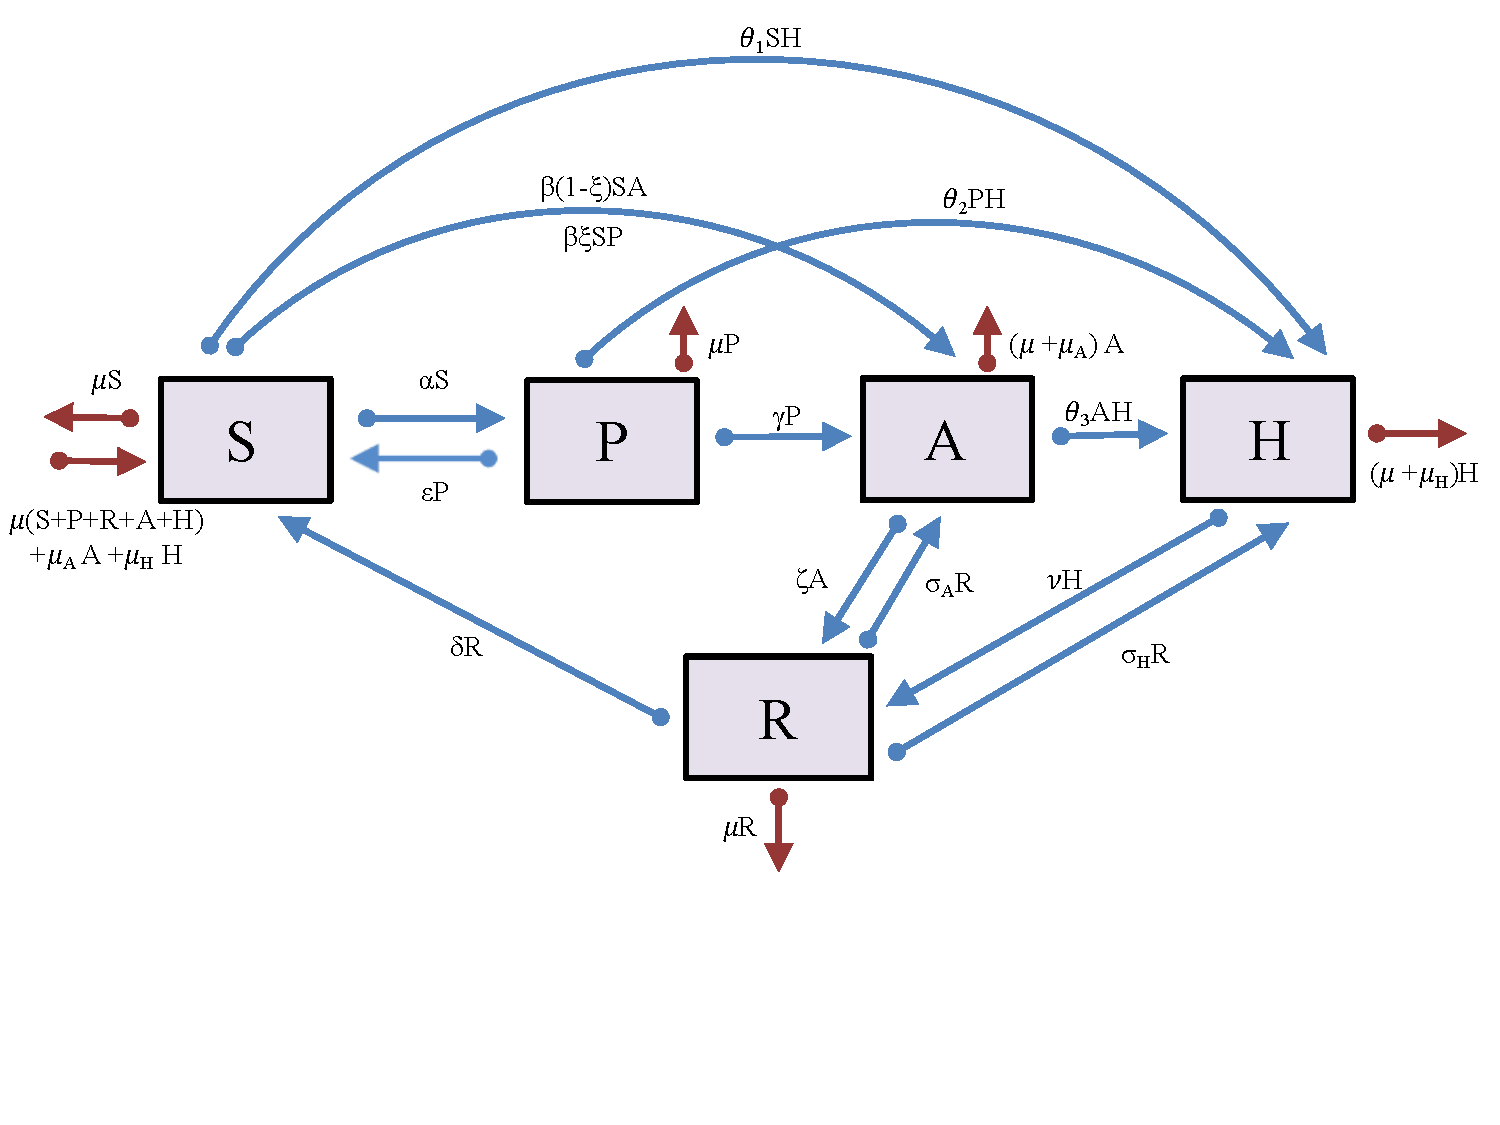
\includegraphics[height=7.5cm, width=12.8cm]{heroin_schematic.pdf} \hspace*{4.5cm}
\begin{center}
$\alpha S$: prescription rate 
\end{center}
\end{frame}


\begin{frame}
\frametitle{}
\vspace{-.28cm}
\hspace*{-1.08cm} 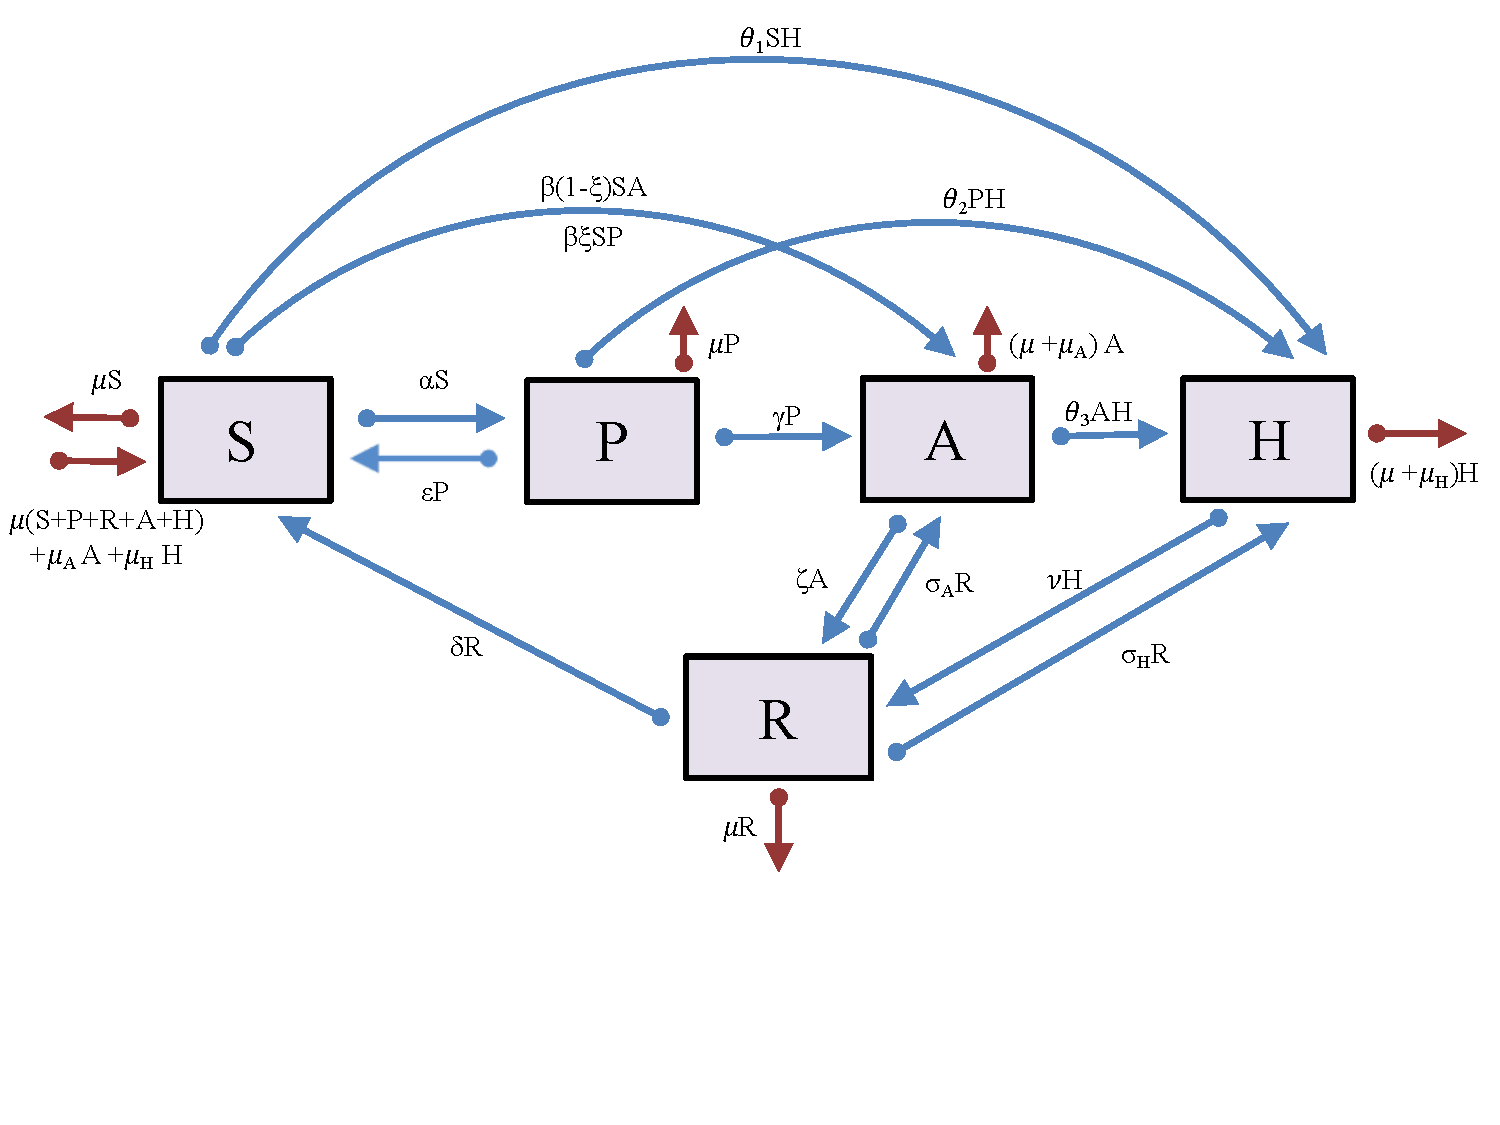
\includegraphics[height=7.5cm, width=12.8cm]{heroin_schematic.pdf} \hspace*{4.5cm}
\begin{center}
$\beta(1-\xi)SA$: opioid addiction rate by black market drugs/interaction with other addicts 
\end{center}
\end{frame}




\begin{frame}
\frametitle{}
\vspace{-.52cm}
\hspace*{-1.08cm} 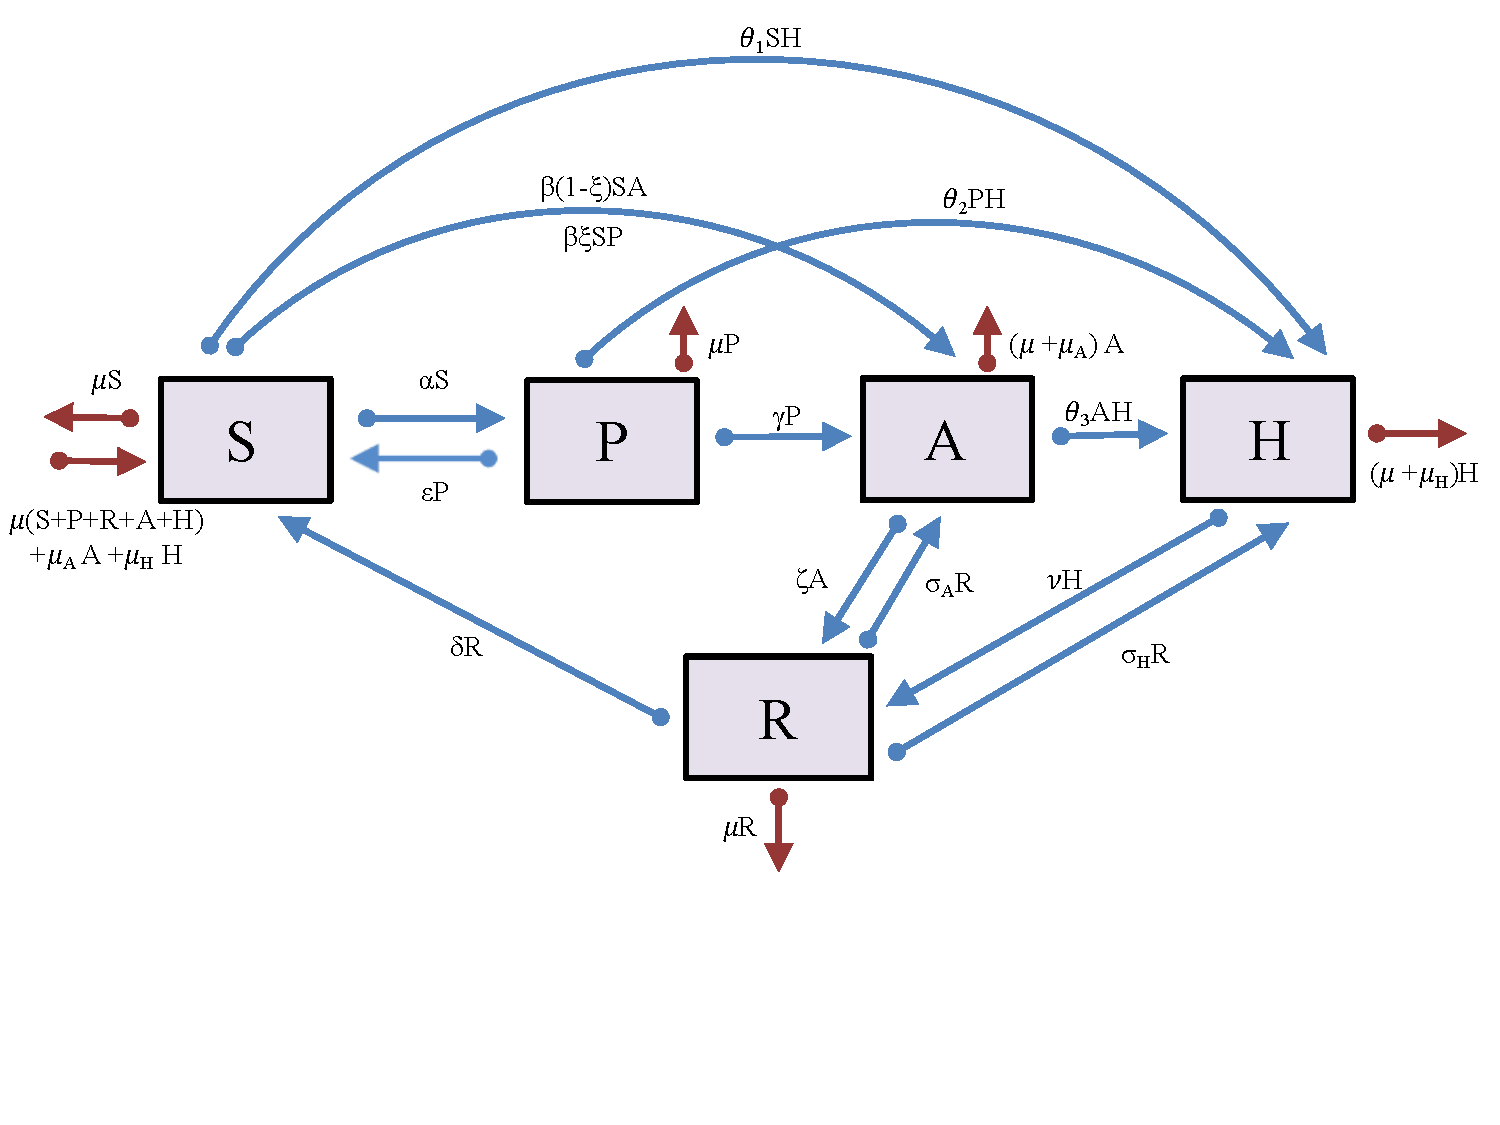
\includegraphics[height=7.5cm, width=12.8cm]{heroin_schematic.pdf} \hspace*{4.5cm}
\begin{center}
$\beta \xi SP$ : opioid addiction rate by obtaining extra prescription opioids 
\end{center}
\end{frame}




\begin{frame}
\frametitle{}
\vspace{-.28cm}
\hspace*{-1.08cm} 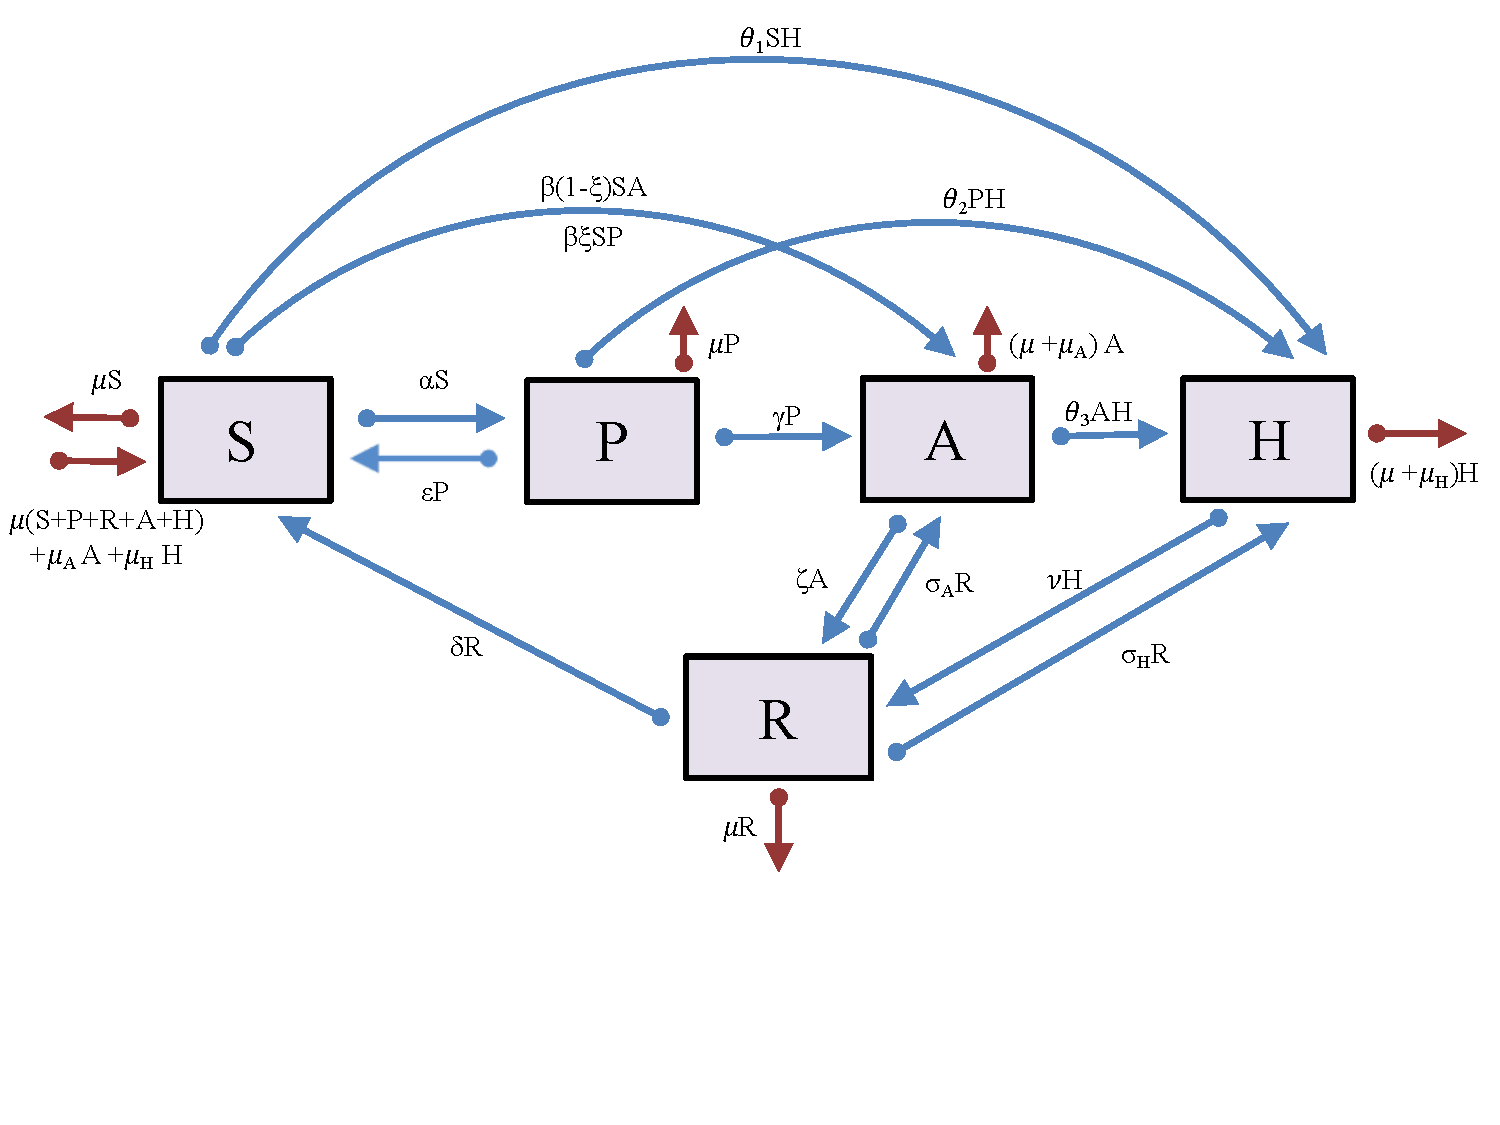
\includegraphics[height=7.5cm, width=12.8cm]{heroin_schematic.pdf} \hspace*{4.5cm}
\begin{center}
$\theta_1 SH$: rate of addiction to heroin by black market availability/ interaction with other users 
\end{center}
\end{frame}




\begin{frame}
\frametitle{}
\vspace{-.52cm}
\hspace*{-1.08cm} 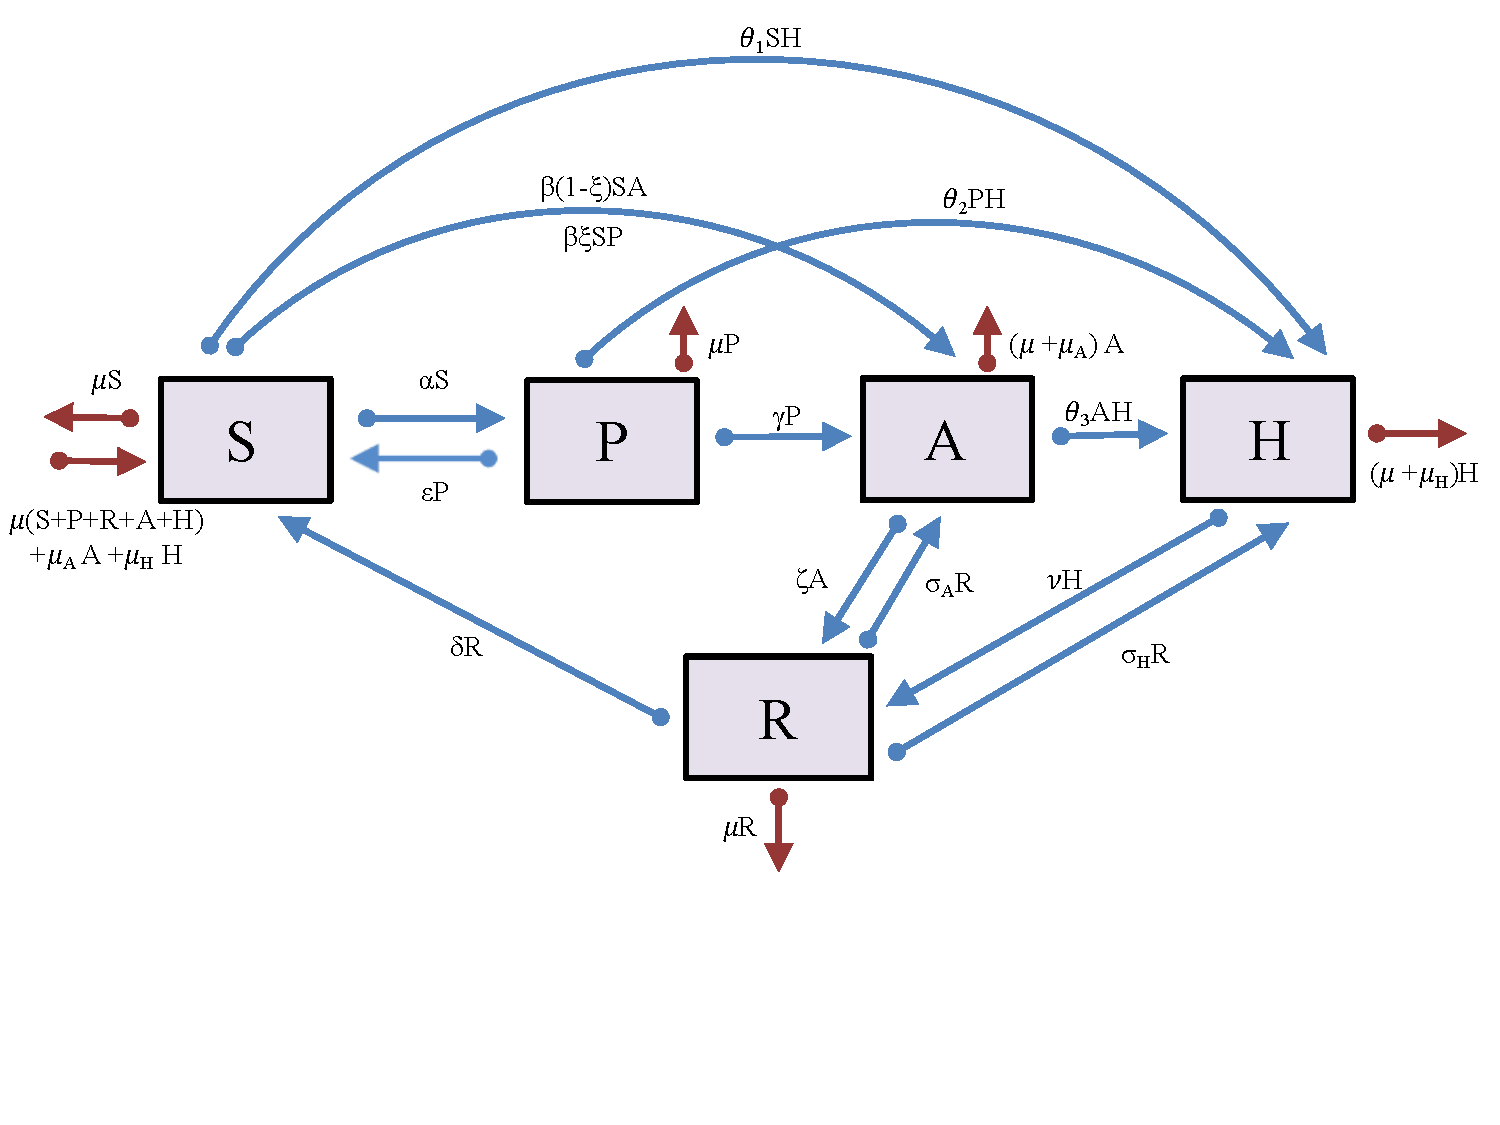
\includegraphics[height=7.5cm, width=12.8cm]{heroin_schematic.pdf} \hspace*{4.5cm}
\begin{center}
$\epsilon P$: rate of non-addicted opioid prescribed users back to susceptible
\end{center}
\end{frame}




\begin{frame}
\frametitle{}
\vspace{-.52cm}
\hspace*{-1.08cm} 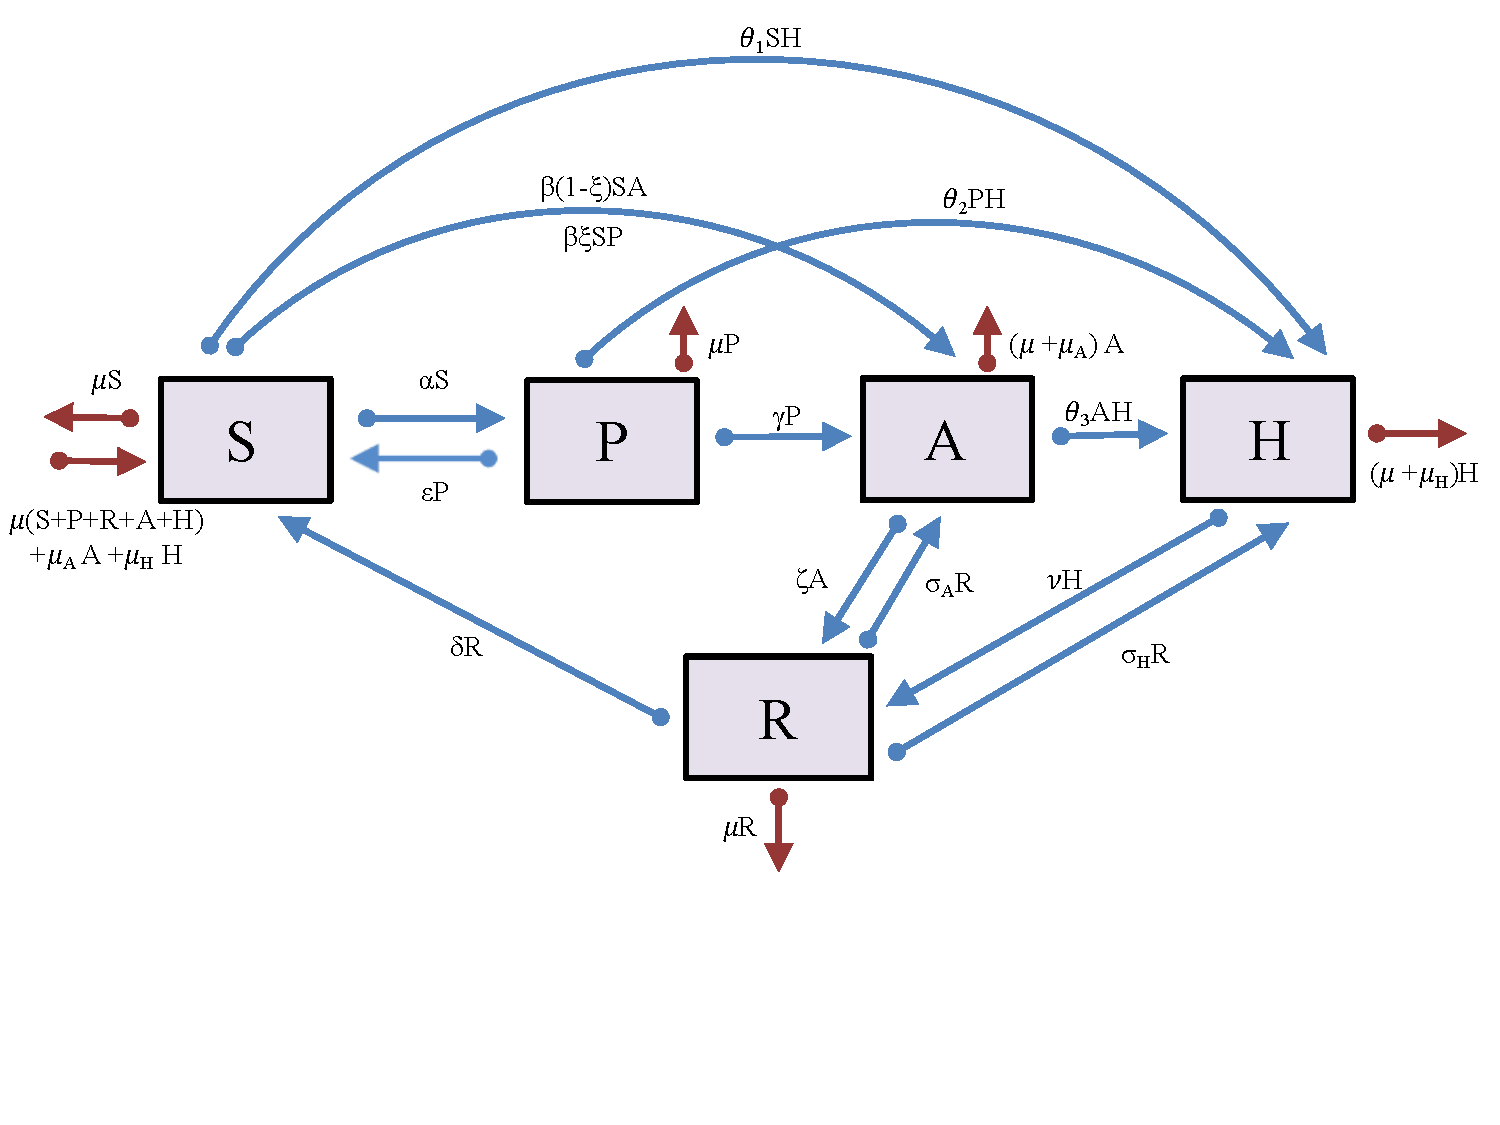
\includegraphics[height=7.5cm, width=12.8cm]{heroin_schematic.pdf} \hspace*{4.5cm}
\begin{center}
$\delta R$: rate of opioid and heroin addicts successfully finishing treatment
\end{center}
\end{frame}




\begin{frame}
\frametitle{}
\vspace{-.52cm}
\hspace*{-1.08cm} 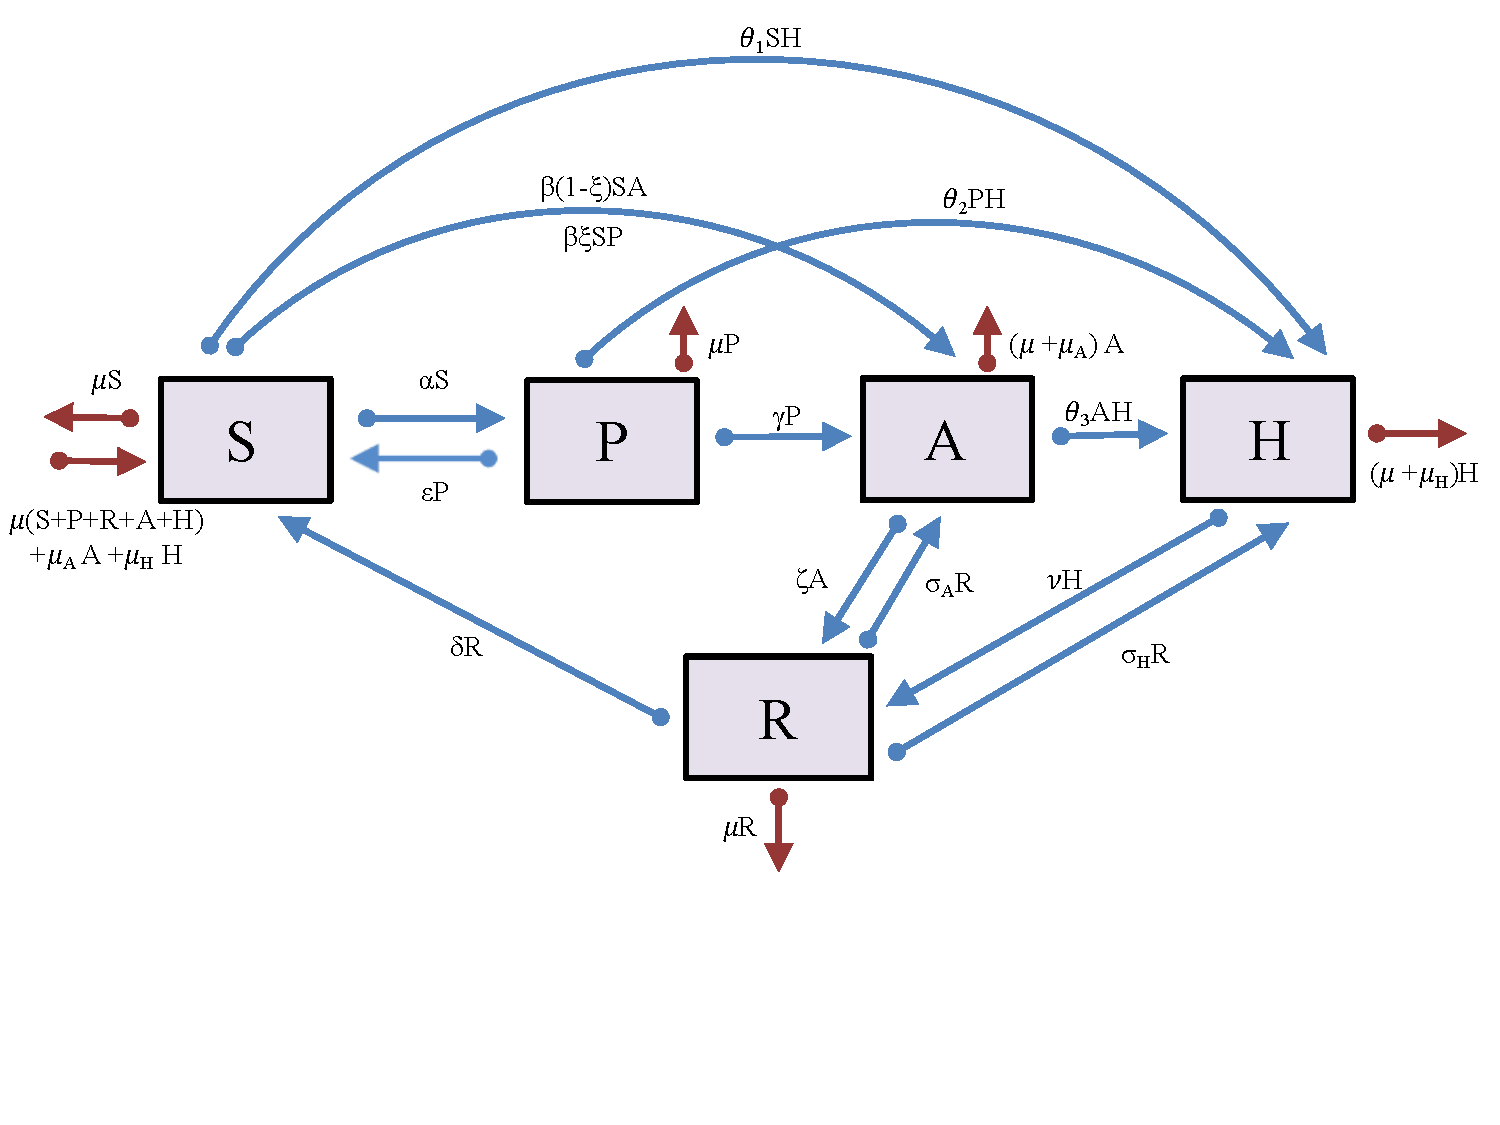
\includegraphics[height=7.5cm, width=12.8cm]{heroin_schematic.pdf} \hspace*{4.5cm}
\begin{center}
 $\mu S$, $\mu P$, $\mu A$, $\mu H$, $\mu R$: natural death rates
\end{center}
\end{frame}




\begin{frame}
\frametitle{}
\vspace{-.52cm}
\hspace*{-1.08cm} 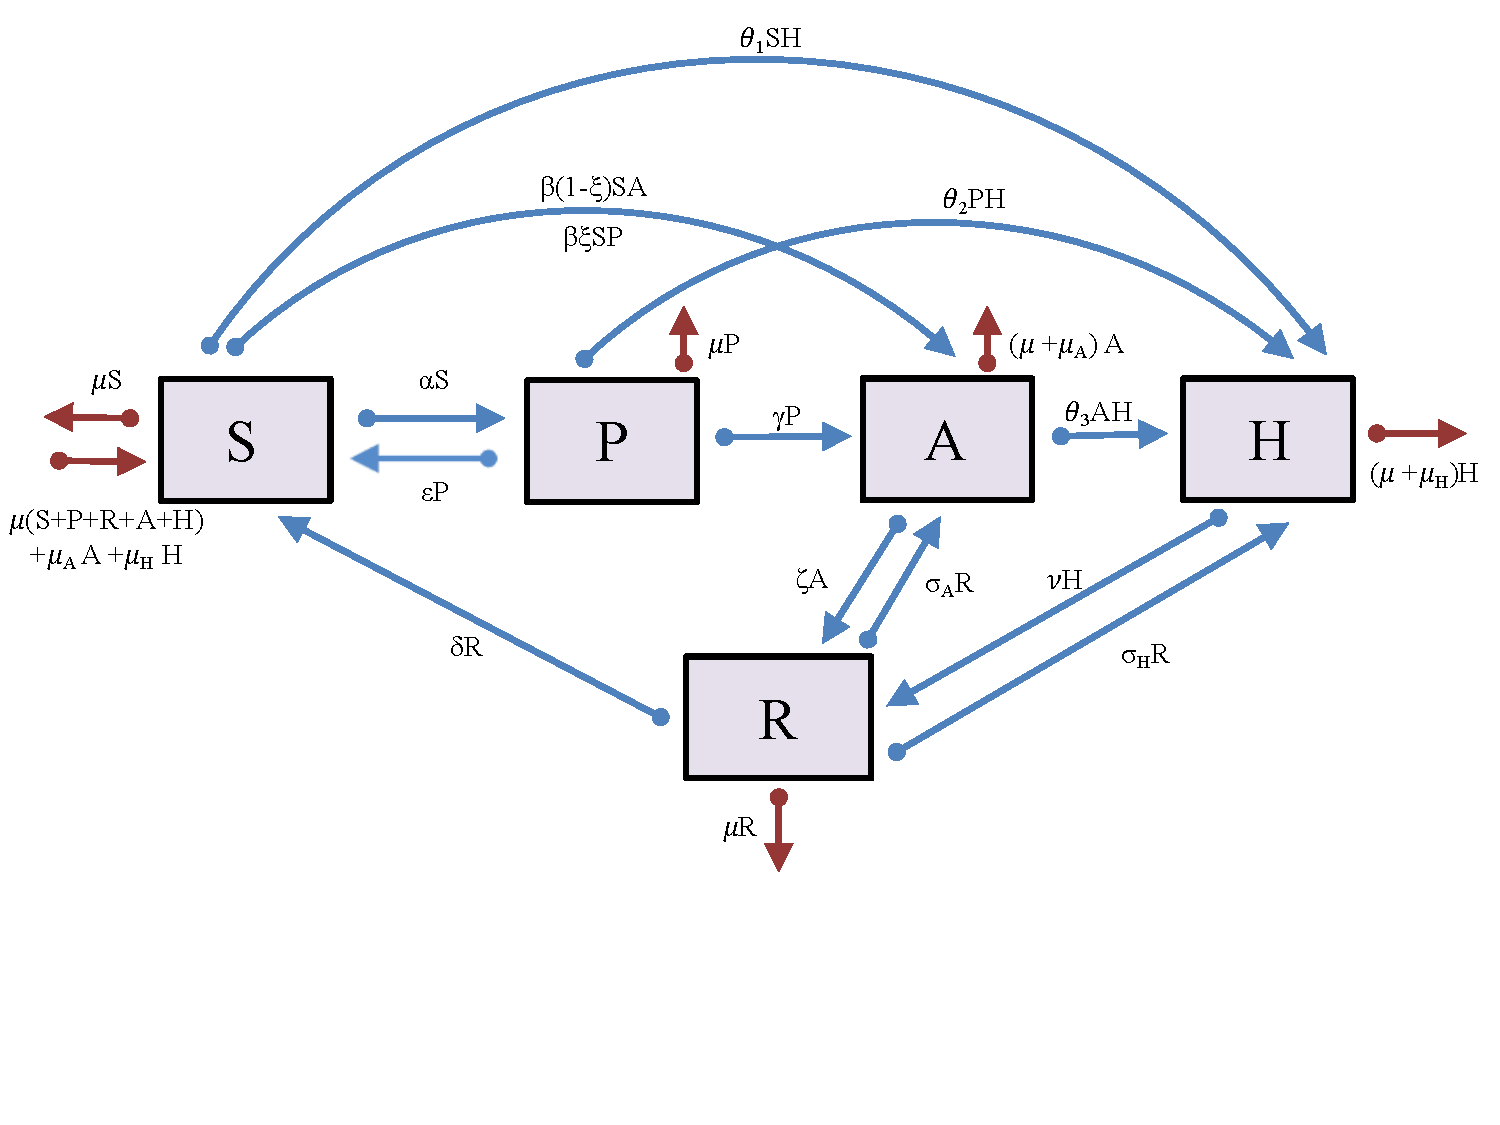
\includegraphics[height=7.5cm, width=12.8cm]{heroin_schematic.pdf} \hspace*{4.5cm}
\begin{center}
$\mu_A A$: opioid addict overdose death rate 
\end{center}
\end{frame}




\begin{frame}
\frametitle{}
\vspace{-.52cm}
\hspace*{-1.08cm} 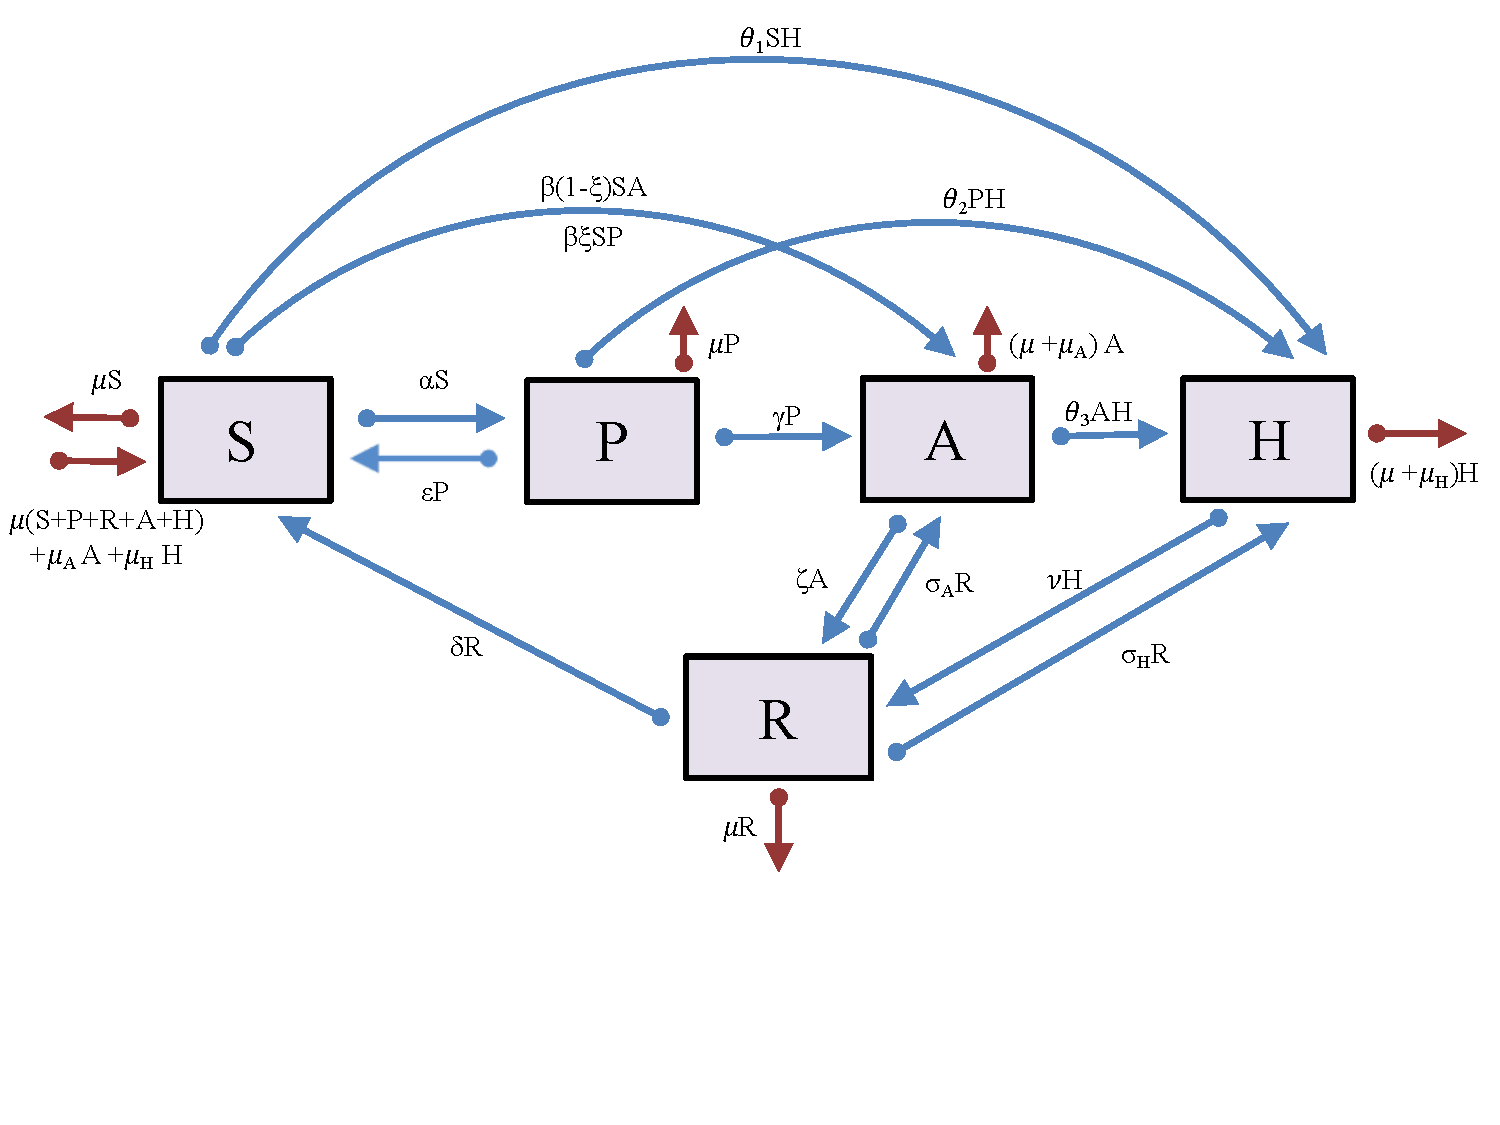
\includegraphics[height=7.5cm, width=12.8cm]{heroin_schematic.pdf} \hspace*{4.5cm}
\begin{center}
$\mu_H H$: heroin user overdose death rate 
\end{center}
\end{frame}




\begin{frame}
\frametitle{}
\vspace{-.52cm}
\hspace*{-1.08cm} 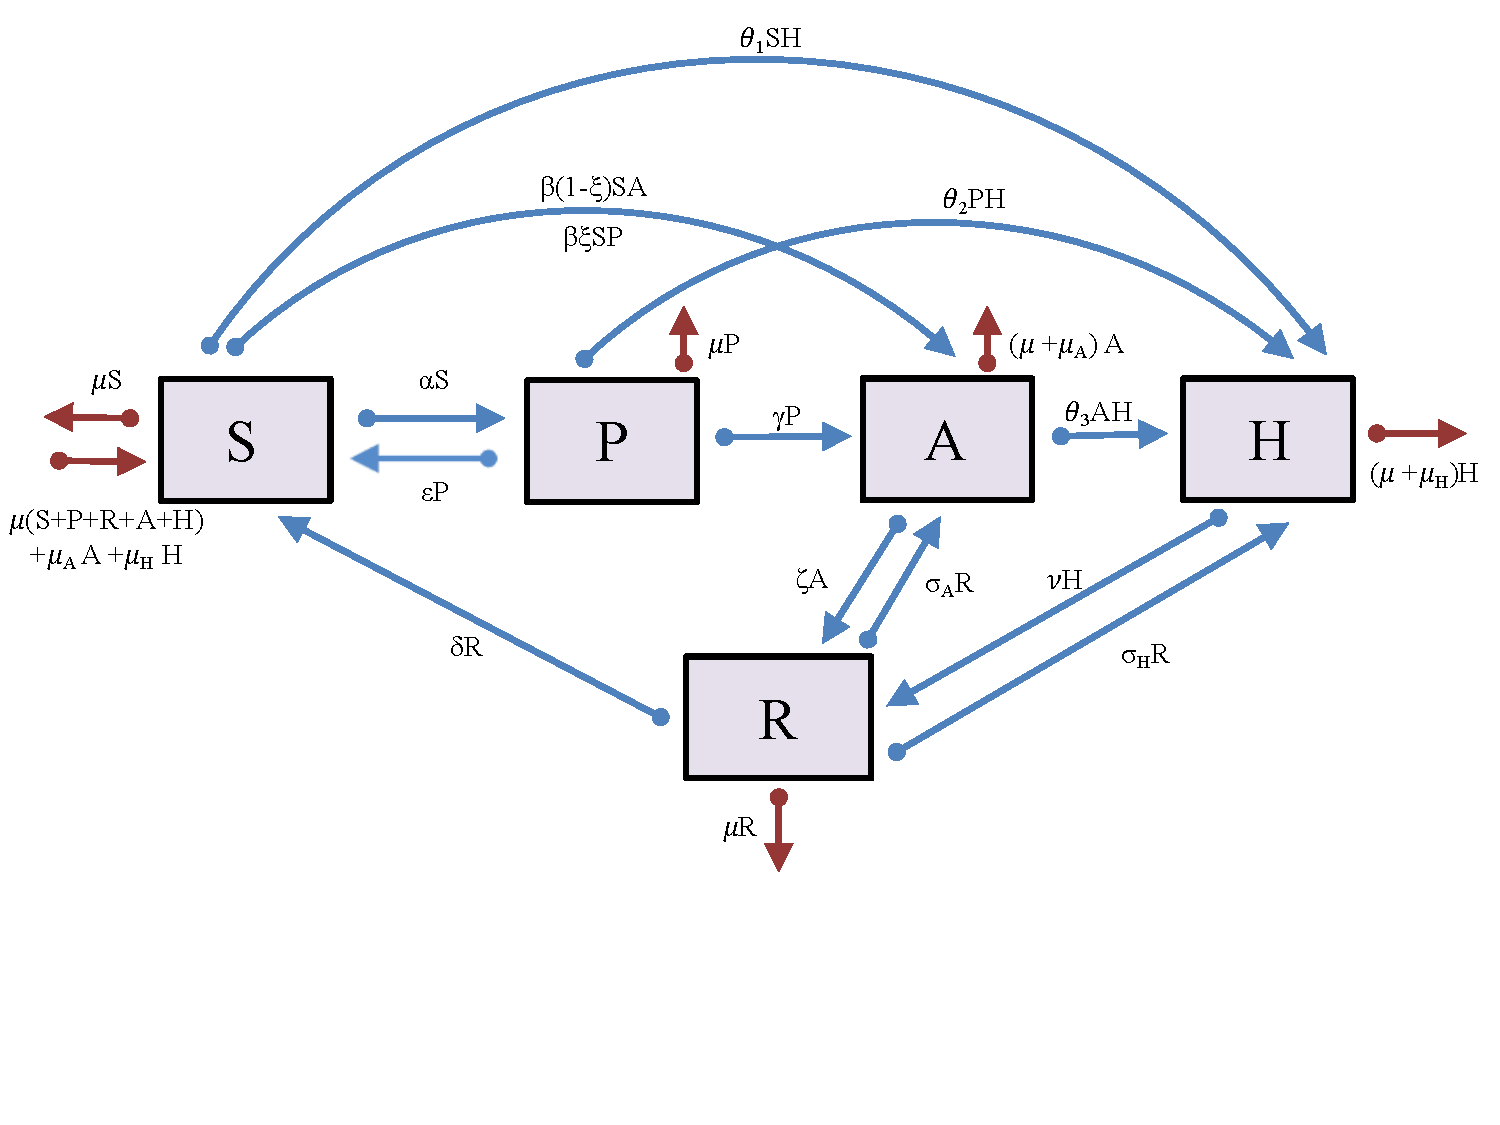
\includegraphics[height=7.5cm, width=12.8cm]{heroin_schematic.pdf} \hspace*{4.5cm}
\begin{center}
$\gamma P$: rate of opioid addiction for prescribed users
\end{center}
\end{frame}




\begin{frame}
\frametitle{}
\vspace{-.52cm}
\hspace*{-1.08cm} 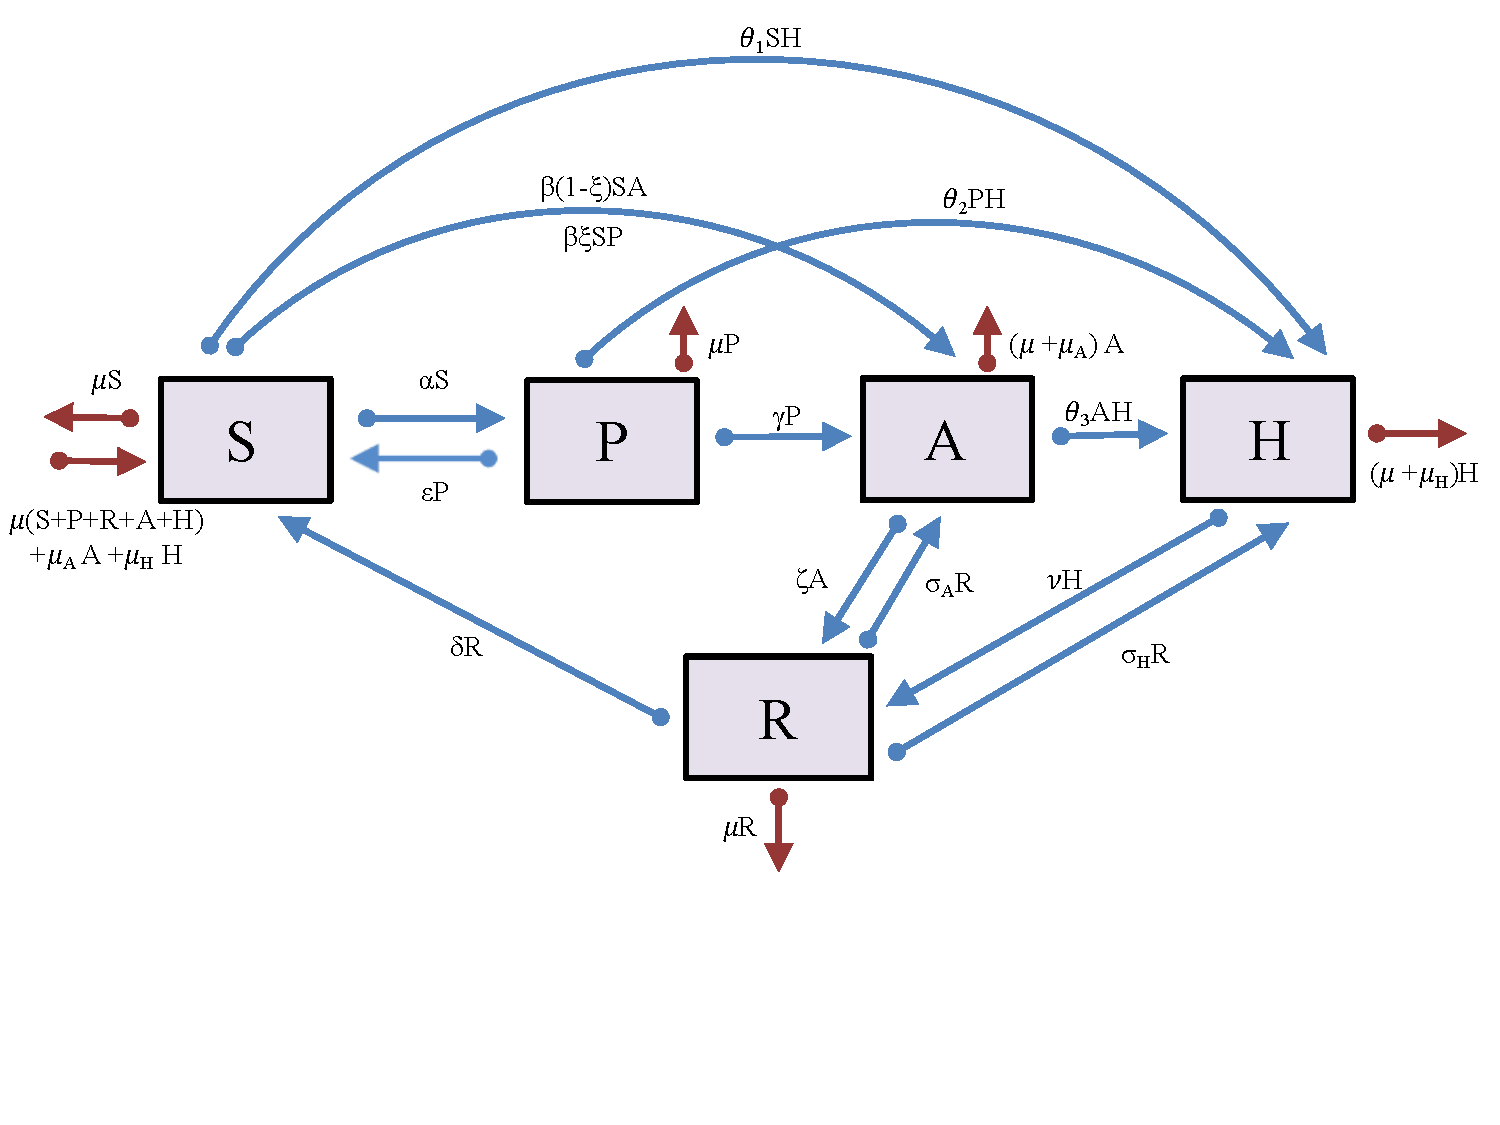
\includegraphics[height=7.5cm, width=12.8cm]{heroin_schematic.pdf} \hspace*{4.5cm}\begin{center}
$\theta_2 PH$: rate of heroin addiction for prescribed users 
\end{center}
\end{frame}




\begin{frame}
\frametitle{}
\vspace{-.52cm}
\hspace*{-1.08cm} 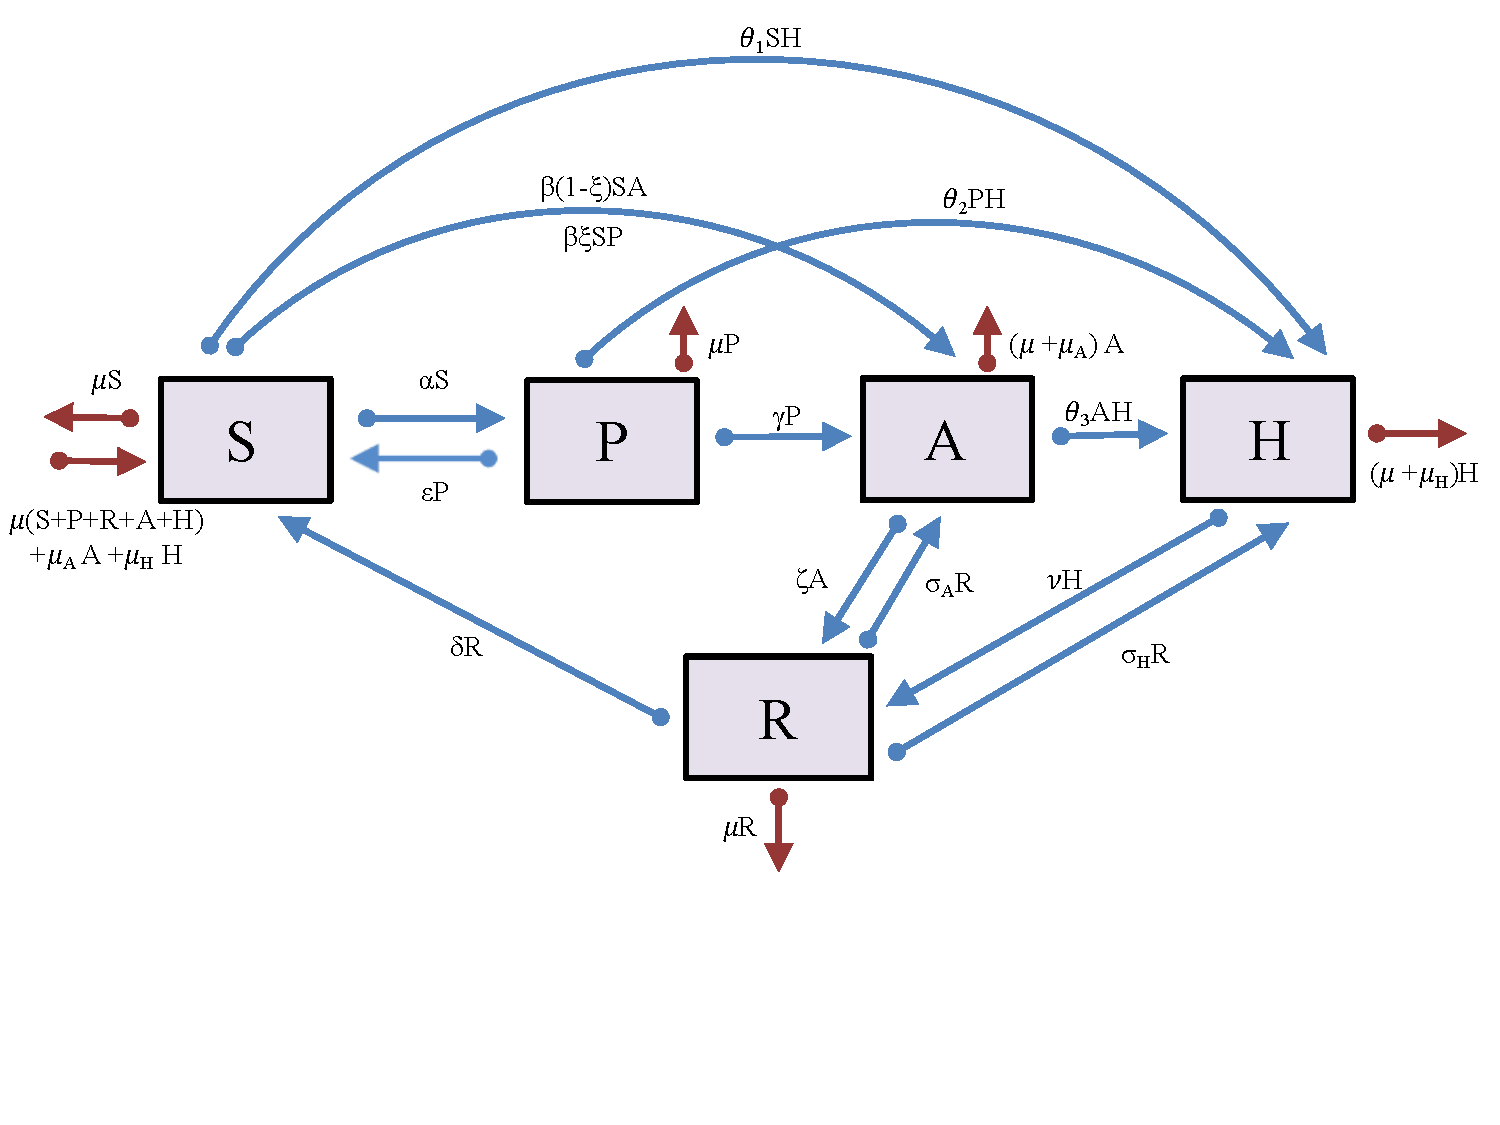
\includegraphics[height=7.5cm, width=12.8cm]{heroin_schematic.pdf} \hspace*{4.5cm}\begin{center}
$\sigma_A R$: transition rate from treatment into the opioid addicted class  
\end{center}
\end{frame}




\begin{frame}
\frametitle{}
\vspace{-.52cm}
\hspace*{-1.08cm} 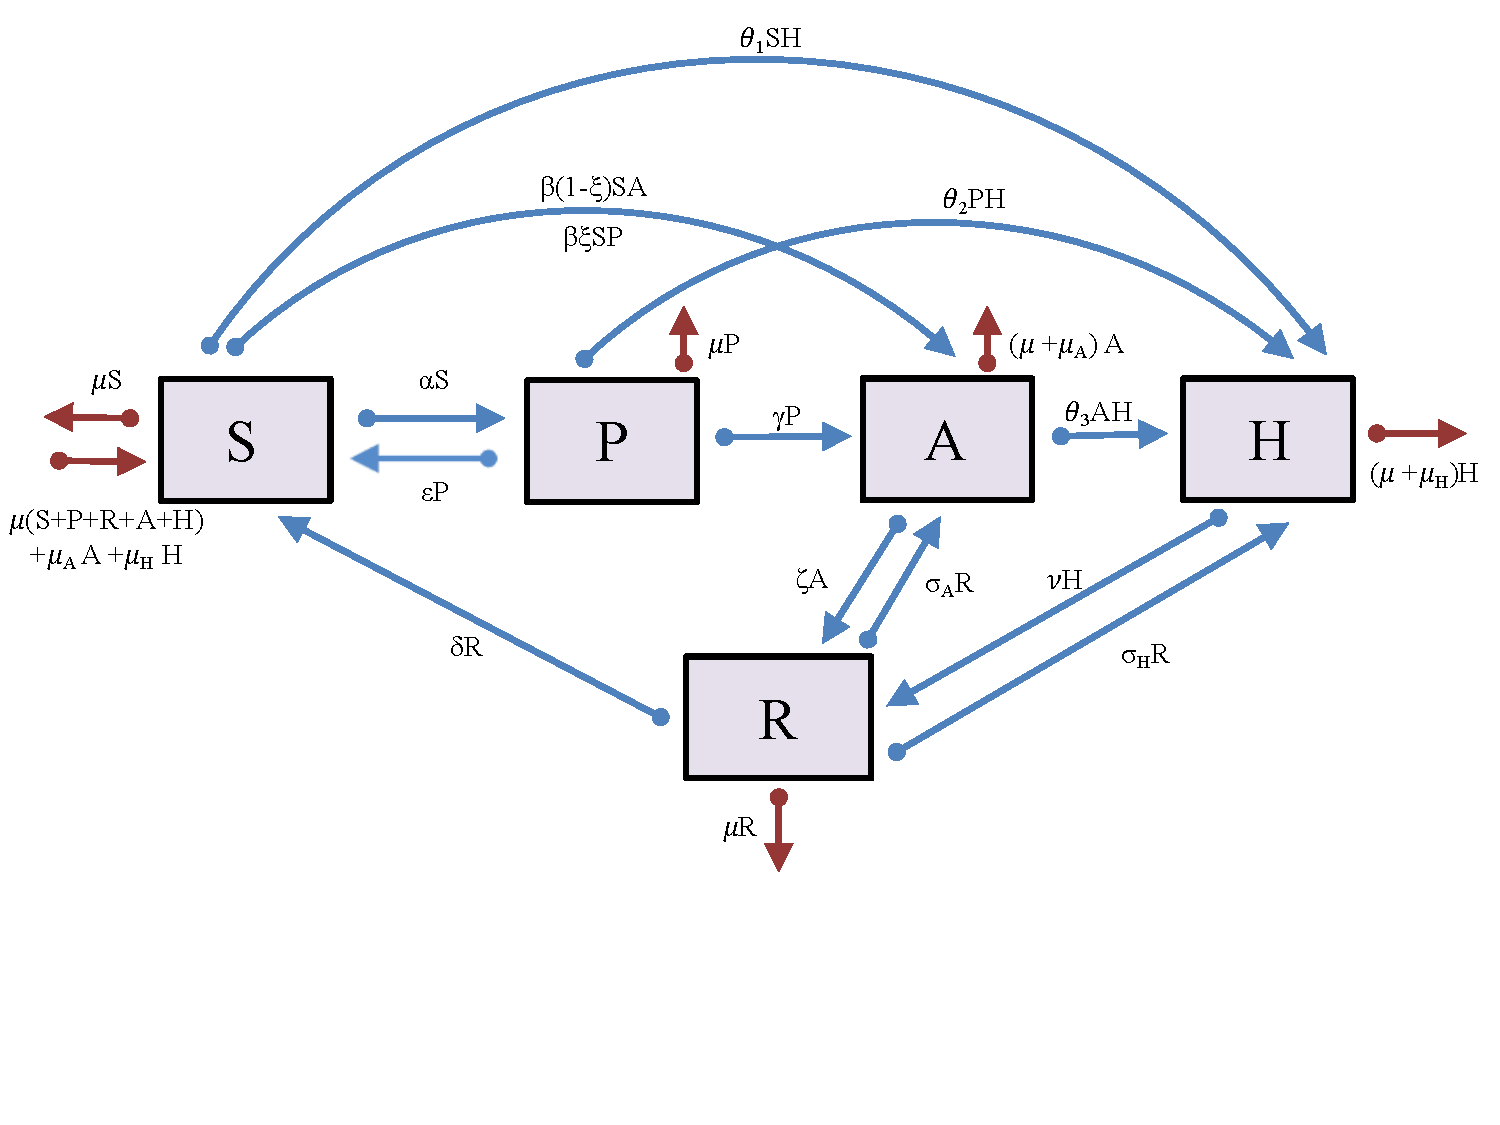
\includegraphics[height=7.5cm, width=12.8cm]{heroin_schematic.pdf} \hspace*{4.5cm}
\begin{center}
$\sigma_H R$: transition rate from treatment into the heroin addicted class 
\end{center}
\end{frame}




\begin{frame}
\frametitle{}
\vspace{-.52cm}
\hspace*{-1.08cm} 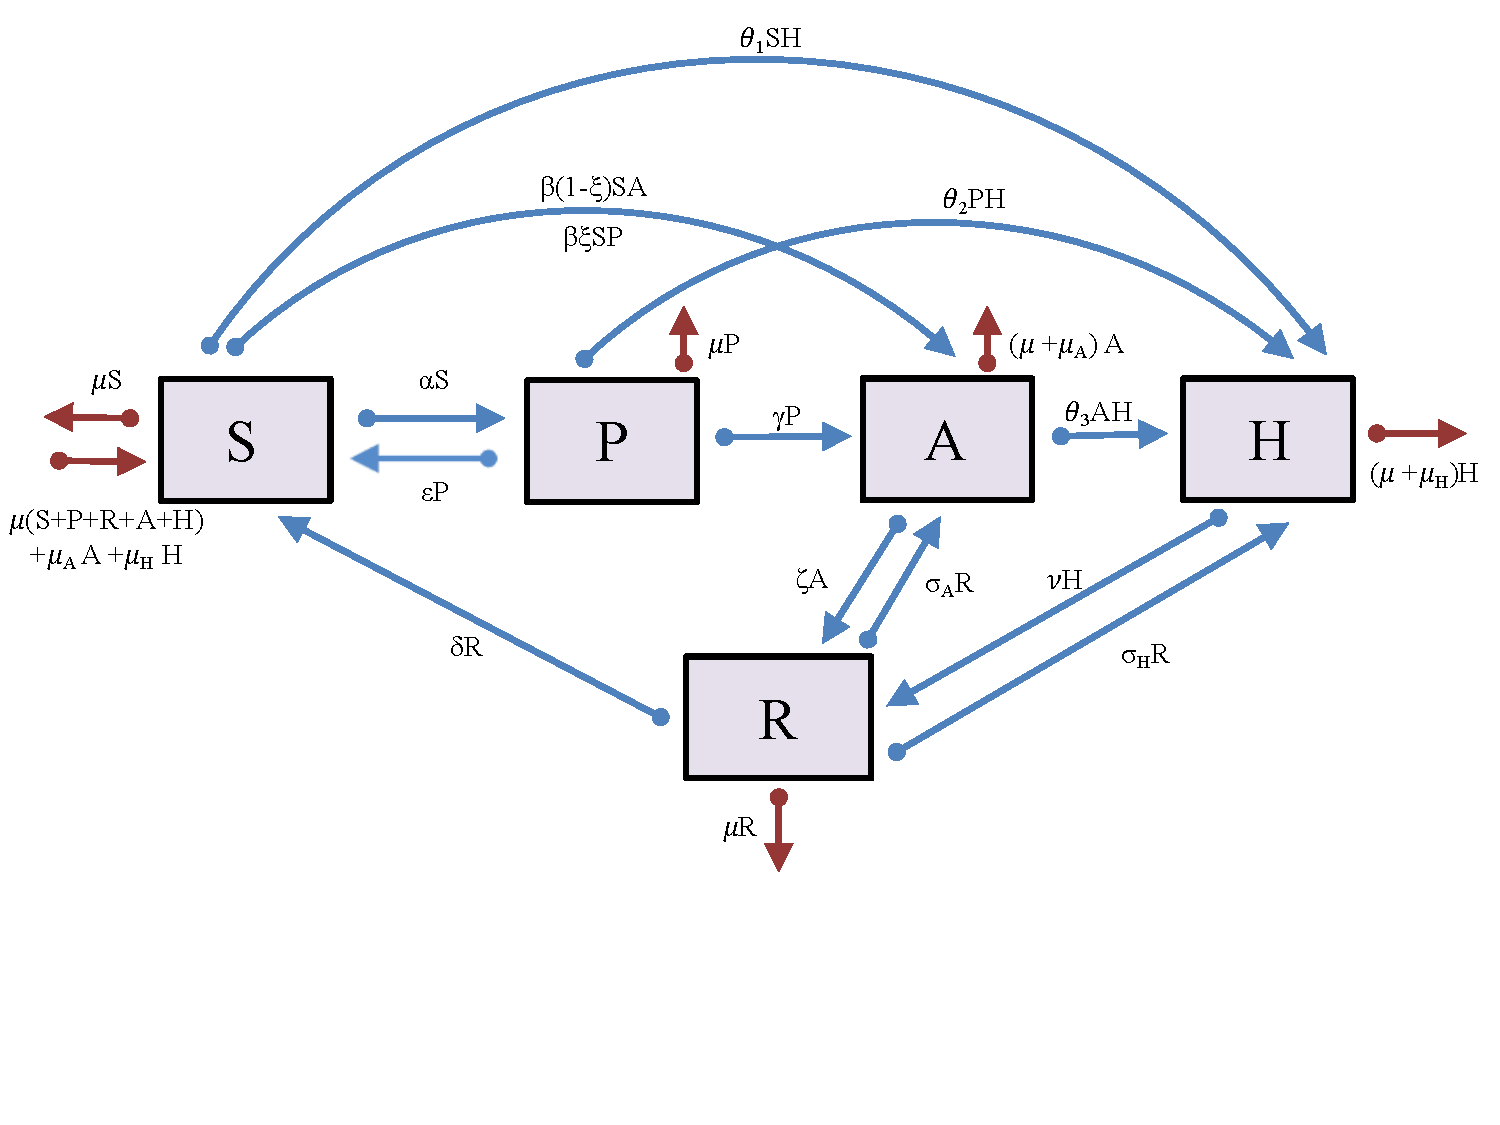
\includegraphics[height=7.5cm, width=12.8cm]{heroin_schematic.pdf} \hspace*{4.5cm}
\begin{center}
$\zeta A$: rate addicted opioid users enter treatment
\end{center}
\end{frame}




\begin{frame}
\frametitle{}
\vspace{-.56cm}
\hspace*{-1.08cm} 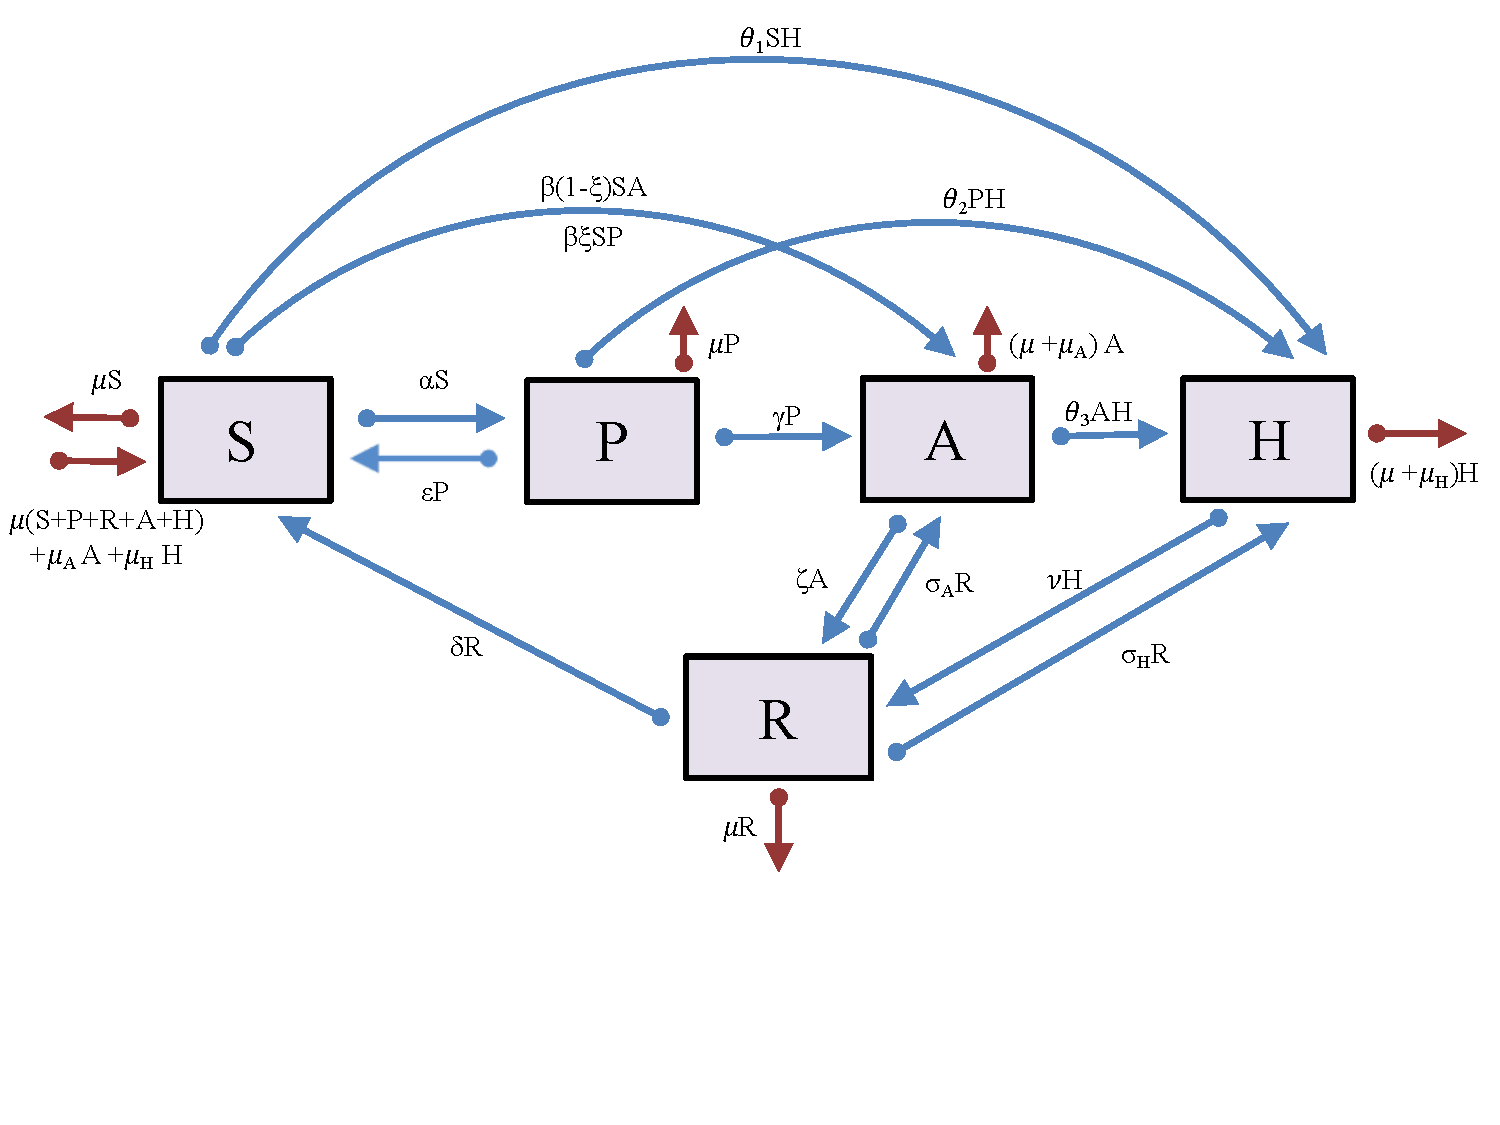
\includegraphics[height=7.5cm, width=12.8cm]{heroin_schematic.pdf} \hspace*{4.5cm}
\begin{center}
$\nu H$: rate heroin users enter treatment 
\end{center}
\end{frame}




\begin{frame}
\frametitle{}
\vspace{-.52cm}
\hspace*{-1.08cm} 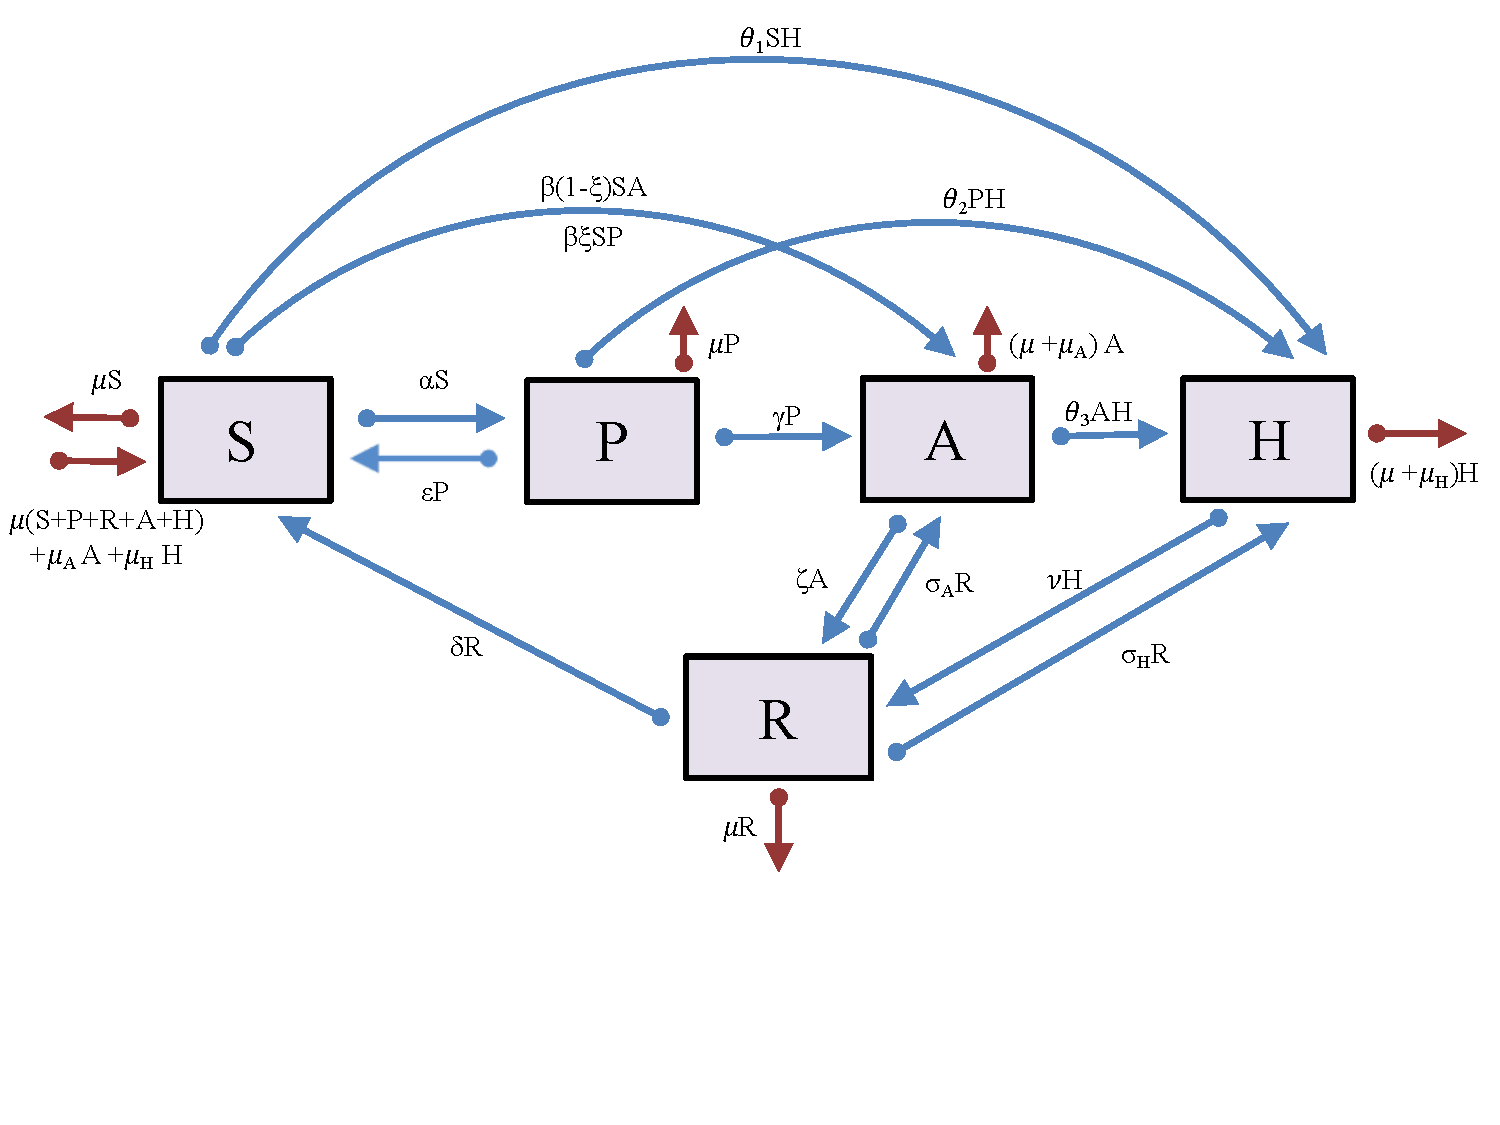
\includegraphics[height=7.5cm, width=12.8cm]{heroin_schematic.pdf} \hspace*{4.5cm}
\begin{center}
$\theta_3 AH$: heroin addiction rate from opioid addicted 
\end{center}
\end{frame}







\begin{comment}
\begin{frame}
\frametitle{Model Formulation}
\begin{columns}
\begin{column}{0.5\textwidth} 
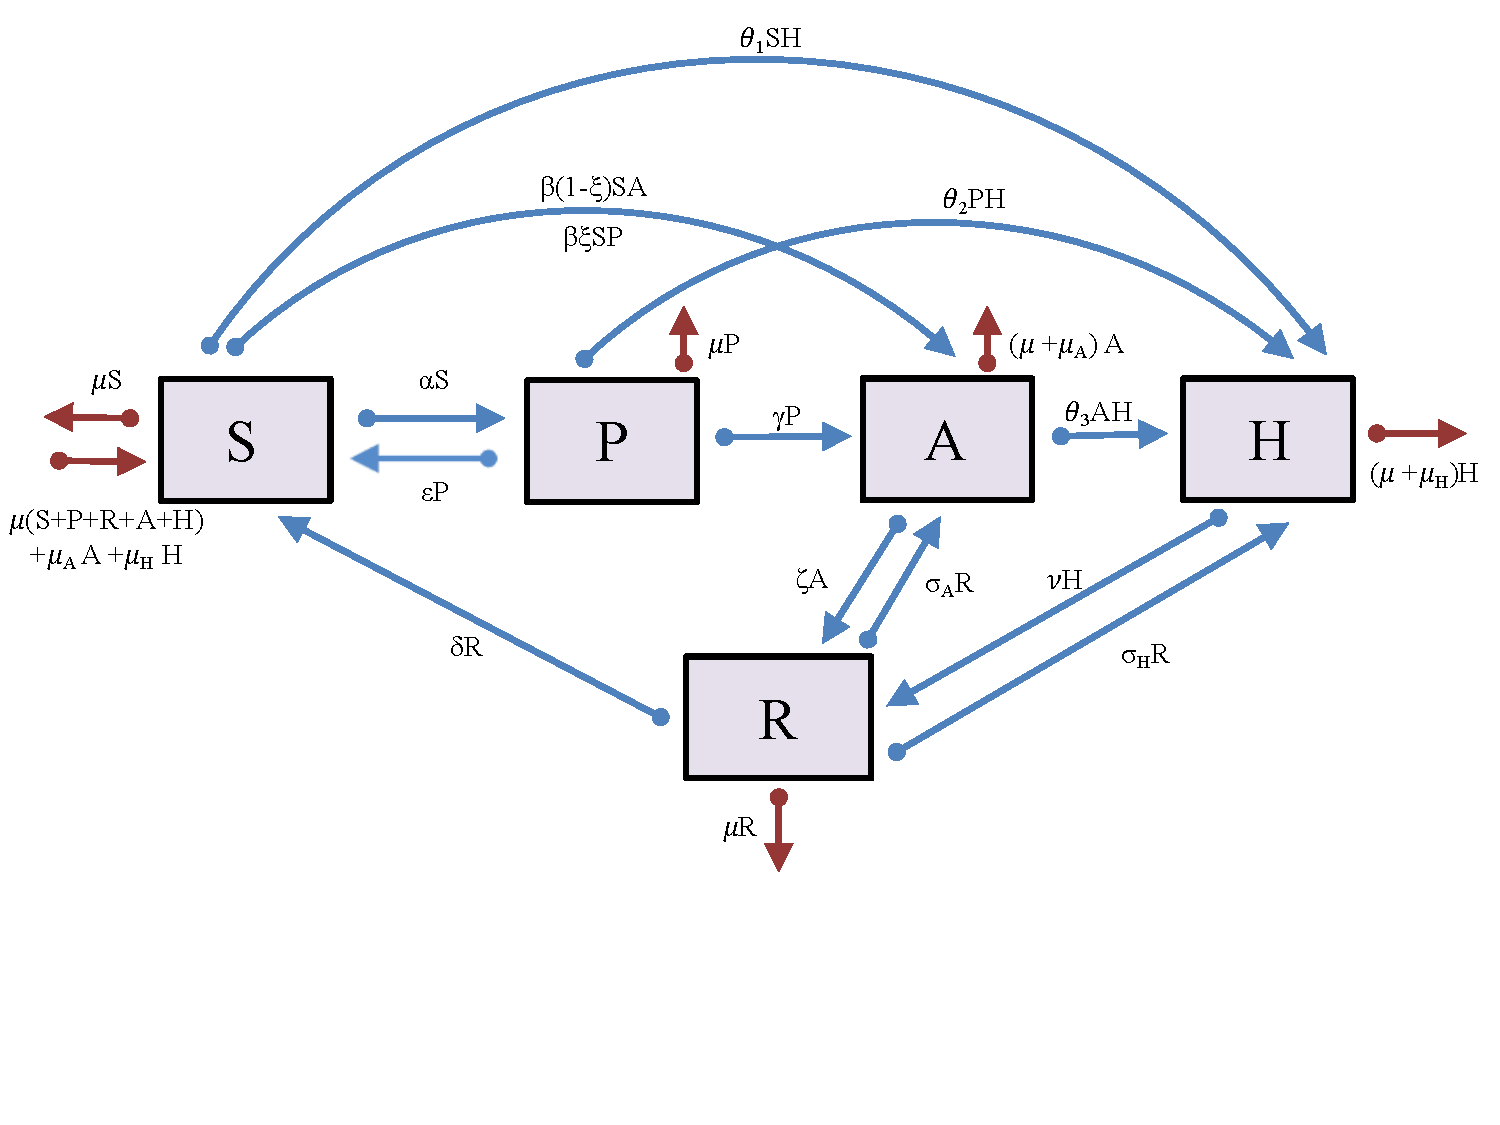
\includegraphics[height=4cm, width=7cm]{heroin_schematic.pdf}
\end{column}
\begin{column}{0.5\textwidth}
\begin{itemize}
\vspace{-0.2cm} 
\item<1>Parameters:
\begin{enumerate}[-]
\item<1> $\alpha S$: prescription rate 
%\item<1> $\beta$ : total probability of opioid addiction by non-prescription means
\item<1> $\beta(1-\xi)SA$: opioid addiction rate by black market drugs/interaction with other addicts 
\item<1>  $\beta \xi SP$ : opioid addiction rate by obtaining extra prescription opioids 
\end{enumerate}
\end{itemize}
\end{column}
\end{columns}
\end{frame}
\end{comment}

\begin{comment}
\begin{frame}
\frametitle{Model Formulation}
\begin{columns}
\begin{column}{0.5\textwidth} 
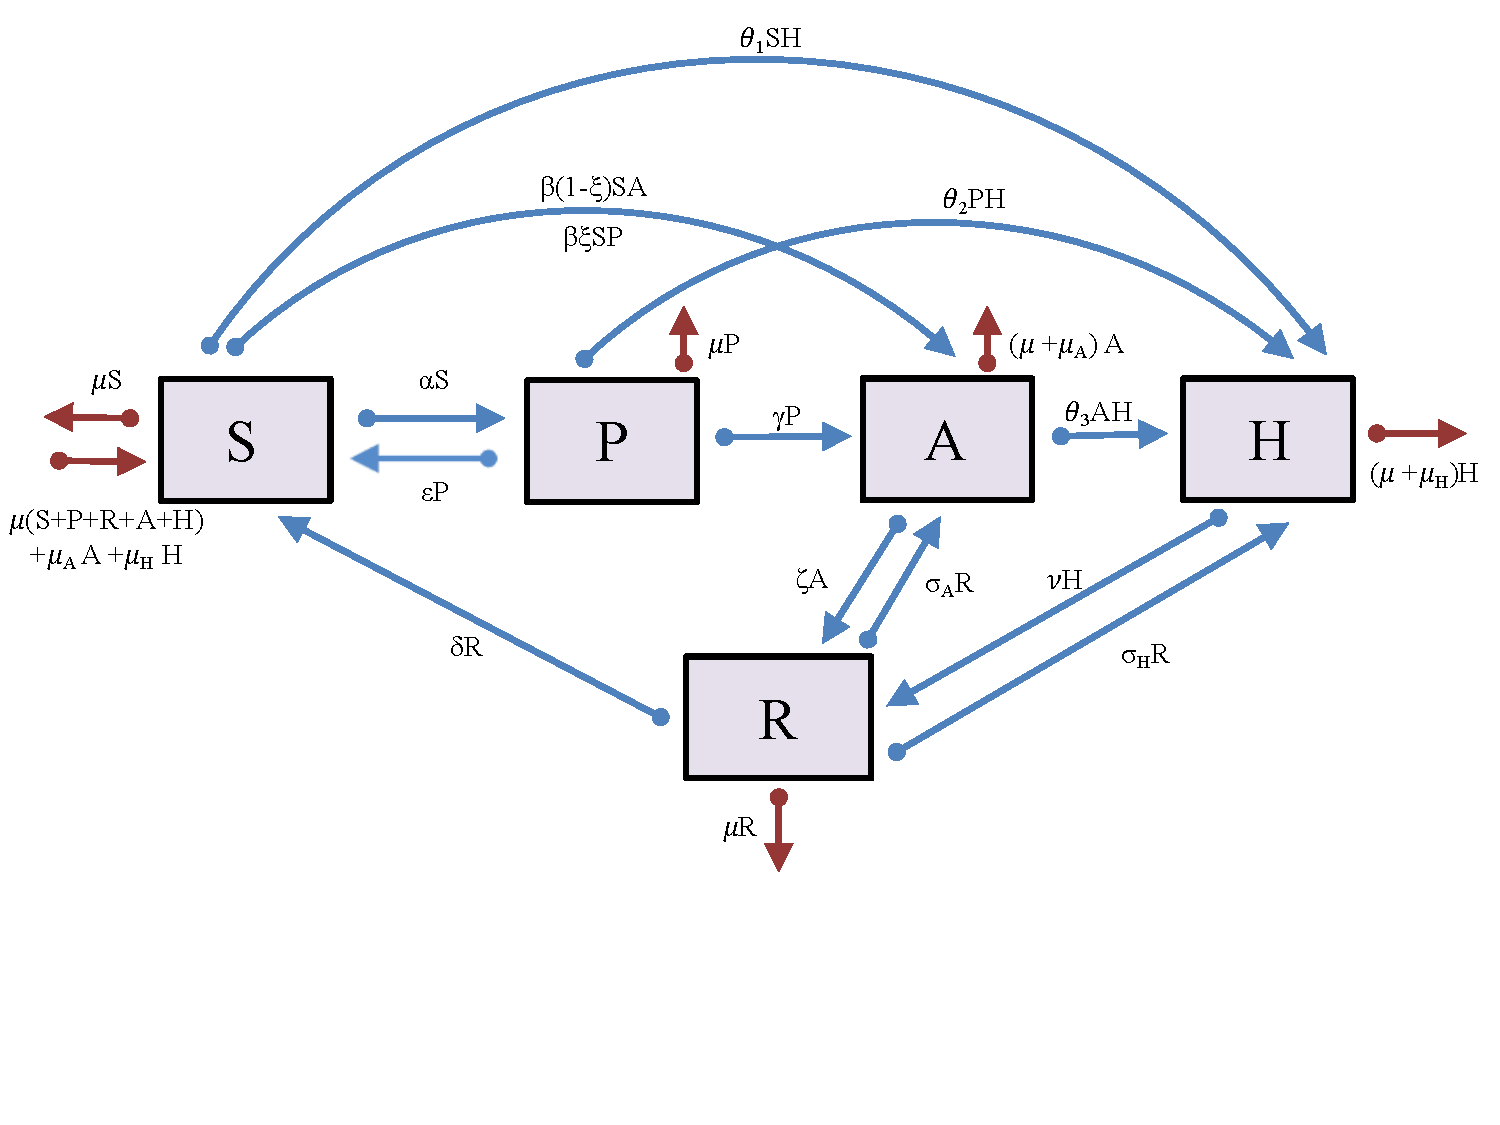
\includegraphics[height=4cm, width=7cm]{heroin_schematic.pdf}
\end{column}
\begin{column}{0.5\textwidth}
\vspace{-0.6cm} 
\begin{itemize}
\item<1>Parameters:
\begin{enumerate}[-]
\vspace{.1cm}
\item<1> $\theta_1 SH$: rate of addiction to heroin by black market availability/ interaction with other users 
\vspace{.1cm}
\item<1>$\epsilon P$: rate of non-addicted opioid prescribed users back to susceptible
\vspace{.1cm} 
\item<1>$\delta R$: rate of opioid and heroin addicts successfully finishing treatment
\end{enumerate}
\end{itemize}
\end{column}
\end{columns}
\end{frame}
\end{comment}


\begin{comment}
\begin{frame}
\frametitle{Model Formulation}
\begin{columns}
\begin{column}{0.5\textwidth} 
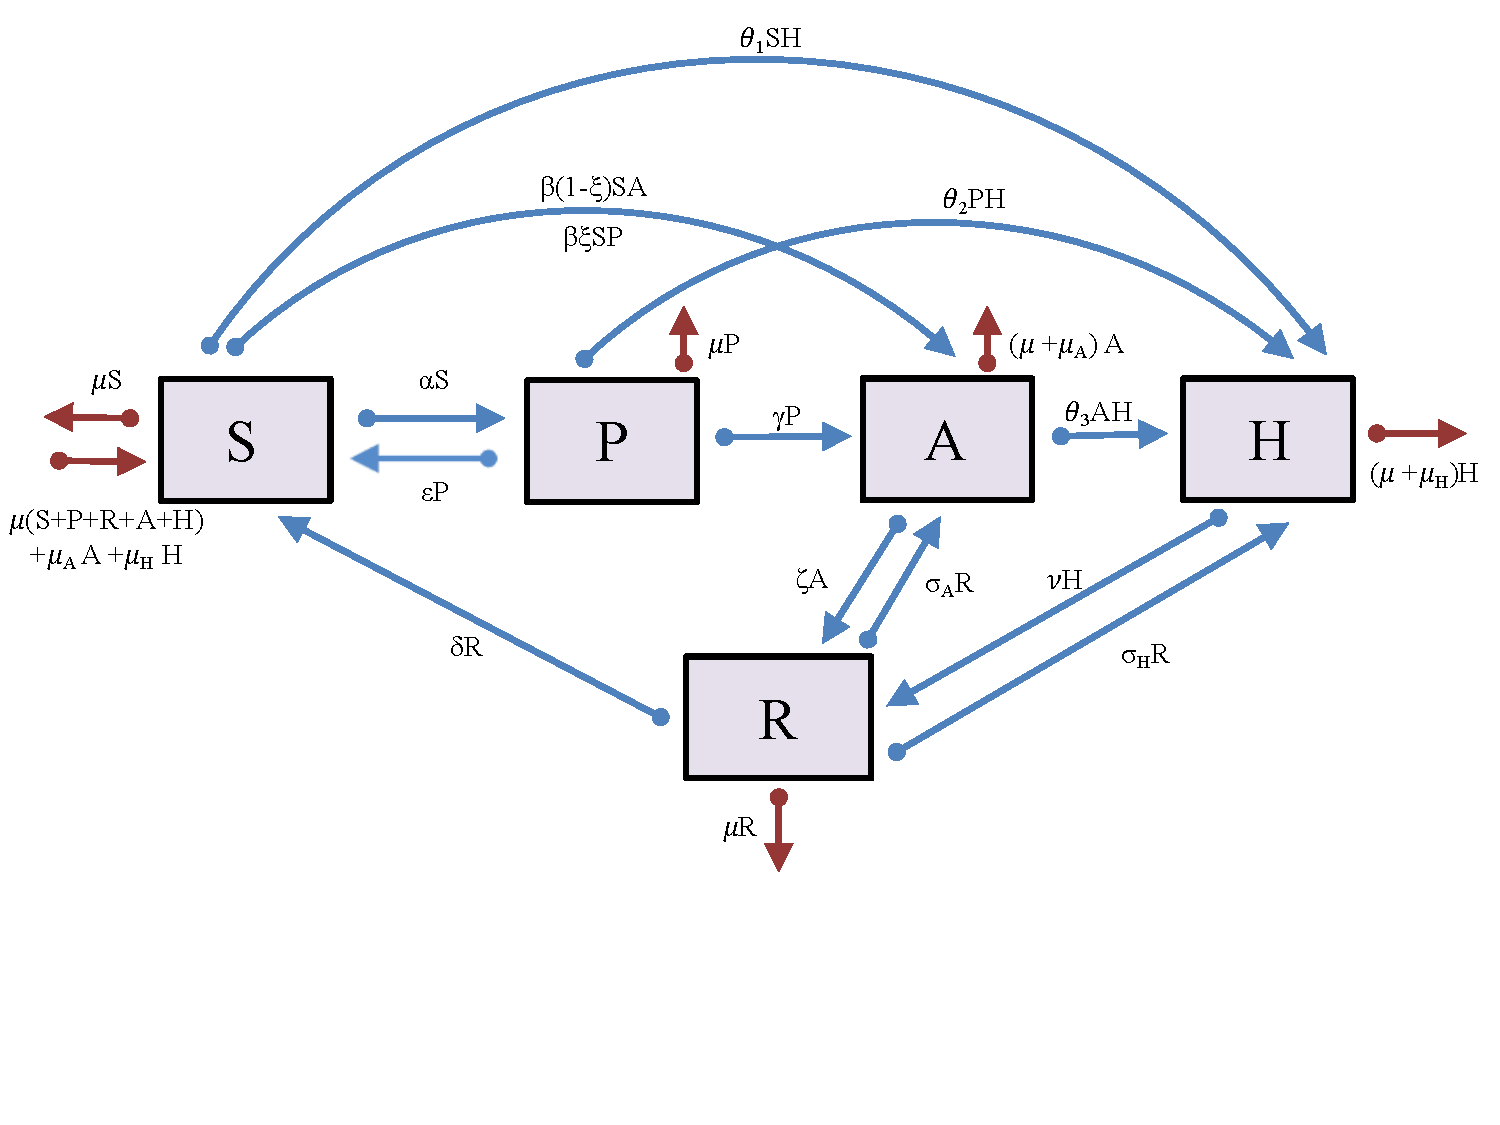
\includegraphics[height=4cm, width=7cm]{heroin_schematic.pdf}
\end{column}
\begin{column}{0.5\textwidth}

\vspace{-0.7cm} 
\begin{itemize}
 \item<1> Parameters:
\begin{enumerate}[-]
\item<1>  $\mu S$, $\mu P$, $\mu A$, $\mu H$, $\mu R$: natural death rates
\vspace{.1cm} 
\item<1> $\mu_A A$: opioid addict overdose death rate 
\vspace{.1cm} 
\item<1> $\mu_H H$: heroin user overdose death rate 
\vspace{.1cm} 
\item<1>$\gamma P$: rate of opioid addiction for prescribed users
\vspace{.1cm} 
\item<1> $\theta_2 PH$: rate of heroin addiction for prescribed users 
\end{enumerate}
\end{itemize}
\end{column}
\end{columns}
\end{frame}
\end{comment}

\begin{comment}
\begin{frame}
\frametitle{Model Formulation}
\begin{columns}
\begin{column}{0.5\textwidth} 
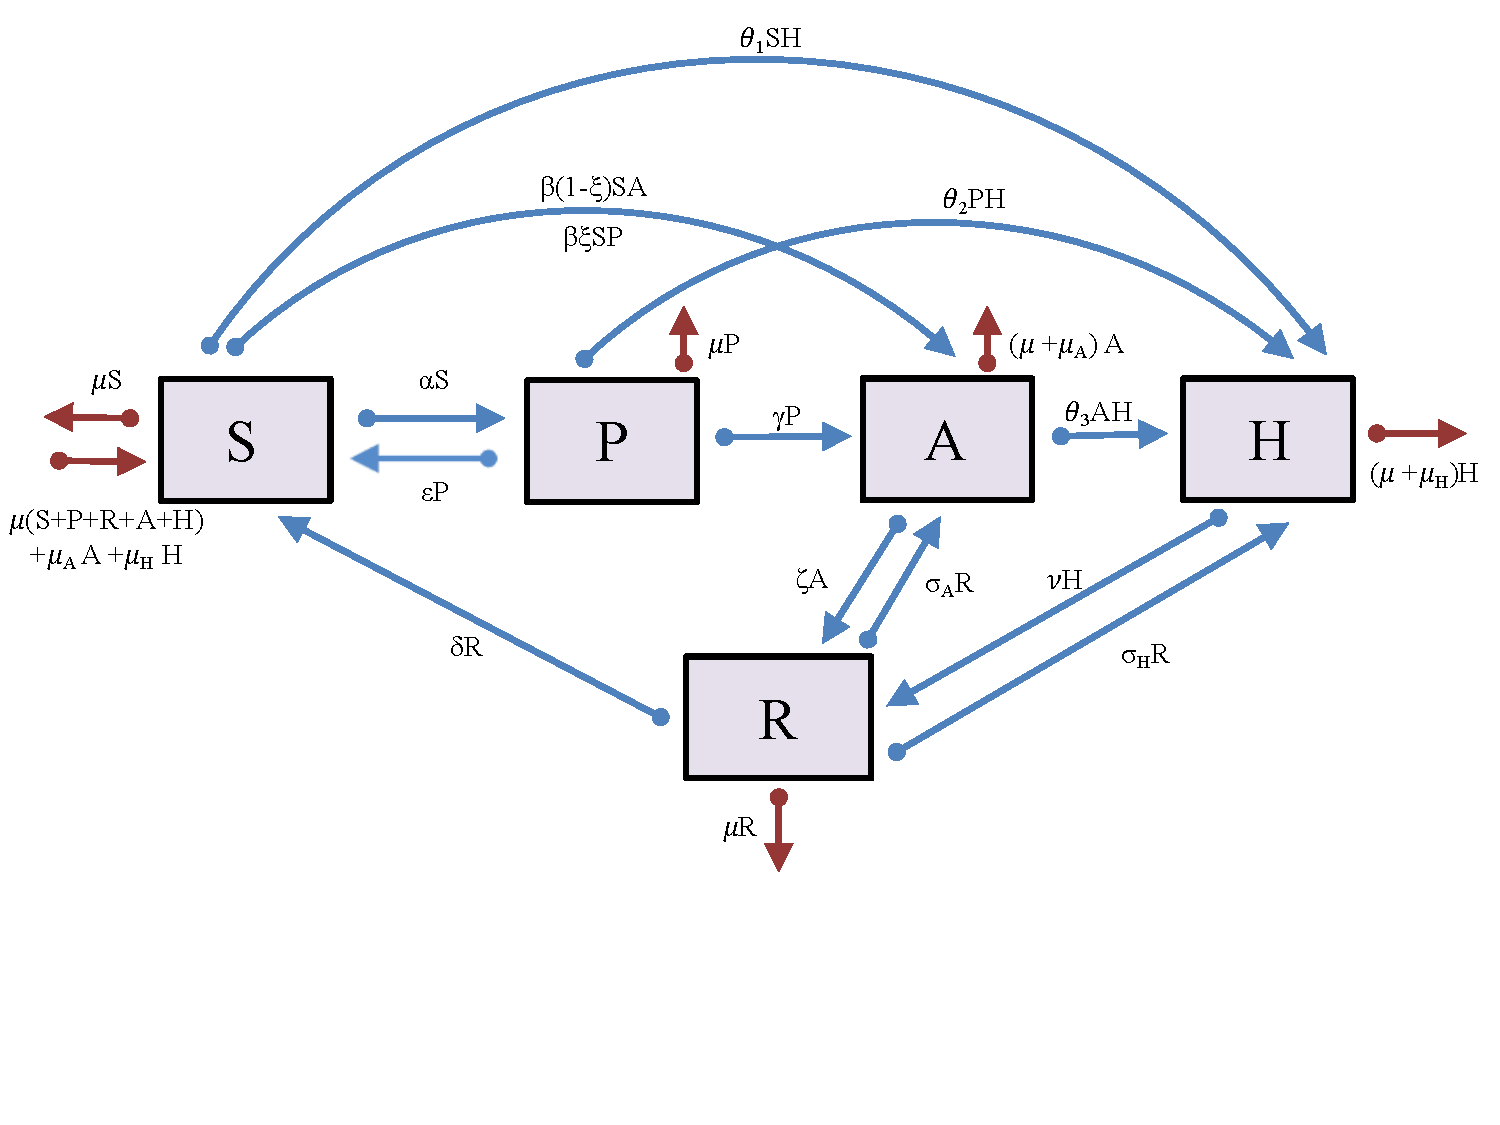
\includegraphics[height=4cm, width=7cm]{heroin_schematic.pdf}
\end{column}
\begin{column}{0.5\textwidth}
\begin{itemize}
\item<1>Parameters:
\begin{enumerate}[-]
\vspace{.2cm}
\item<1> $\sigma_A R$: transition rate from treatment into the opioid addicted class  
\item<1>  $\sigma_H R$: transition rate from treatment into the heroin addicted class 
\item<1> $\zeta A$: rate addicted opioid users enter treatment
\item<1>$\nu H$: rate heroin users enter treatment 
\item<1> $\theta_3 AH$: heroin addiction rate from opioid addicted 
\end{enumerate}
\end{itemize}
\end{column}
\end{columns}
\end{frame}
\end{comment}



\begin{frame}{System of ODEs Model}

\small

$$\dfrac{dS}{dt} = -\alpha S - \beta (1- \xi) SA  -\beta \xi SP- \theta_{1} SH +\epsilon P +\delta R + 
\mu (P+R) + (\mu+\mu_{A})A + (\mu+\mu_{H}) H \hspace{1cm} $$ 


\vspace{.1cm}

$$\dfrac{dP}{dt} = \alpha S - \epsilon P  - \gamma P - \theta_{2}PH- \mu P \hspace{1cm}$$

\vspace{.1cm}

$$\dfrac{dA}{dt} = \gamma P + \sigma_{A} R +\beta (1- \xi) SA  +\beta \xi SP -\zeta A - \theta_{3}AH-(\mu + \mu_{A})A $$ \\

\vspace{.1cm}

$$\dfrac{dH}{dt} = \theta_{1}SH+\theta_{2}PH+\theta_{3}AH + \sigma_{H}R-\nu H-(\mu+\mu_{H})H$$

\vspace{.1cm}

$$\dfrac{dR}{dt} = \zeta A +\nu H -\delta R -\sigma_{A}R-\sigma_{H}R -\mu R$$
\end{frame}

\begin{frame}
\frametitle{Data}
\begin{itemize}
\item<1> We have made contact with individuals in diverse fields in order to obtain data on the opioid and heroin epidemic specifically in Knox County and East Tennessee:
\begin{enumerate}[-]
\vspace{.1cm}
\item<1> Dr. Paul Erwin, Head of the Department of Public Health 
\vspace{.1cm}
\item<1>  Dr. Agricola Odoi, Associate Professor of Epidemiology
\vspace{.1cm}
\item<1> Dr. Kelly Cooper, Director of Clinical Services and Assistant Public Health Officer at the Knox County Health Department 
\end{enumerate}
\end{itemize}
\end{frame}



\section{Heroin Model Analysis}

\begin{frame}
\frametitle{Addiction-Free Equilibrium}
To find the addiction-free equilibrium, require $A=H=R=0 \implies$ 
\[\dfrac{dS}{dt}=0=-\alpha S^* -\beta \xi S^* P^* + \epsilon P^* +\mu P^* \quad\]
\[\dfrac{dP}{dt}=0=\alpha S^* - \epsilon P^* -\gamma P^* - \mu P^* \quad\]
\[\dfrac{dA}{dt}=0=\gamma P^* + \beta \xi S^* P^*.   \quad\]
\begin{itemize}
\item<1> Note: 
\begin{enumerate}[-]
\item<1> If $P^*=0$ $\implies$ the only solution is $S^*=P^*=A^*=H^*=R^*=0$, but $S^*+P^*+A^*+H^*+R^*=1$, not possible.
\end{enumerate}
\end{itemize}
\end{frame}
%think about how would know if AFE is stable or unstable 



\begin{frame}
\frametitle{Addiction-Free Equilibrium}
\[0=-\alpha S^* -\beta \xi S^* P^* + \epsilon P^* +\mu P^* \quad\]
\[0=\alpha S^* - \epsilon P^* -\gamma P^* - \mu P^* \quad\]
\[ \cfbox{red}{$0=\gamma P^* + \beta \xi S^* P^*$} \quad\]
\begin{itemize}
\vspace{-.5cm}
\item<1> Solving: 
\begin{enumerate}[-]
\item<1> Will assume $P^* \neq 0 \implies$ $\gamma + \beta \xi S^* =0$ and since all of our parameters and variables are non-negative $\implies$ $\gamma=0$ and either $\beta=0$ or $\xi=0$.
\vspace{.1cm}
\item $\gamma=0$ means that individuals who are prescribed opioids cannot become addicted to opioids. 
\vspace{.1cm}
\item $\xi=0$ means that only black market opioids are available and there are no excess prescription drugs available. 
\vspace{.1cm}
\item $\beta=0$ means that susceptibles are unable to become addicted to opioids at all (less realistic). 
\end{enumerate}
\end{itemize}
\end{frame}




\begin{frame}
\frametitle{Addiction-Free Equilibrium}
\begin{itemize}
\item<1> Solving continued: 
\begin{enumerate}[-]
\item<1> Assuming $\gamma=0=\xi$ to ensure the existence of our addiction-free equilibrium and that $1=S+P+A+H+R$, we calculate the addiction-free equilibrium to be: \\
\[S^*=\frac{\epsilon + \mu}{\alpha + \epsilon +\mu}\quad\]
\[P^*=\frac{\alpha}{\alpha + \epsilon +\mu}\quad\]
\[A^*=0\quad\]
\[H^*=0\quad\]
\[R^*=0\quad\] 
\item Note that enforcing $P^* \neq 0$ implies that $\alpha \neq 0$, as well.
%would require doctor monitoring, for example 
\end{enumerate}
\end{itemize}
\end{frame}


\begin{frame}
\frametitle{Basic Reproduction Number, $\mathscr{R}_0$ }
\begin{itemize}
\item<1>  In general, $\mathscr{R}_0$ gives the expected number of secondary infected cases that result from the introduction of a disease to a susceptible population. 
\vspace{.1cm}
\item<1> Since $\gamma=0$ and $\xi=0$ for addiction-free equilibrium, individuals can become addicted only with interactions with addicted individuals or heroin users so takes the form of an infectious disease $\implies$ can calculate $\mathscr{R}_0$. 
\vspace{.1cm}
\item<1> Our model has three addiction compartments, A, H and R since these all consist of opioid and/or heroin addicted individuals.
\vspace{.1cm}
\item<1> Will utilize the Next Generation Matrix Method in order to calculate $\mathscr{R}_0.$

\end{itemize}
\end{frame}


\begin{frame}
\frametitle{Calculating $\mathscr{R}_0$ }
\begin{itemize}
\item<1> $\gamma=0$ and $\xi=0$ (thus, $\beta \neq 0$) results in: 
$$\dfrac{dS}{dt} = -\alpha S - \beta SA  - \theta_{1} SH +\epsilon P +\delta R +\mu (P+R) + (\mu+\mu_{A})A + (\mu+\mu_{H}) H$$
$$\dfrac{dP}{dt} = \alpha S - \epsilon P  - \theta_{2}PH- \mu P $$
$$\dfrac{dA}{dt} = \sigma_{A} R +\beta SA  -\zeta A - \theta_{3}AH-(\mu + \mu_{A})A $$
$$\dfrac{dH}{dt} = \theta_{1}SH+\theta_{2}PH+\theta_{3}AH + \sigma_{H}R-\nu H-(\mu+\mu_{H})H $$
$$\dfrac{dR}{dt} = \zeta A +\nu H -\delta R -\sigma_{A}R-\sigma_{H}R -\mu R.$$

\end{itemize}
\end{frame}


\begin{frame}
\frametitle{Calculating $\mathscr{R}_0$ }
\begin{itemize}
\item<1>  We may write the differential equations of the addicted compartments, A, H and R as: \\
$$\dfrac{dA}{dt} = \mathscr{F}_{1} (x,y)-\mathscr{V}_{1}(x,y)$$
$$\dfrac{dH}{dt} = \mathscr{F}_{2} (x,y)-\mathscr{V}_{2}(x,y)$$
$$\dfrac{dR}{dt} = \mathscr{F}_{3} (x,y)-\mathscr{V}_{3}(x,y),$$
where $x= {[A\quad H\quad R]}^{T}$, $y= {[S\quad P]}^{T}$, $\mathscr{F}_{i}$ represents rate that new addicted cases contribute to addicted compartment $i$ and $\mathscr{V}_{i}$ represents rate of transitions, i.e. rate the addicted compartment $i$ is decreased by means of death, recovery and progression of the addiction (for $i=1,2,3$). 

\end{itemize}
\end{frame}





\begin{frame}
\frametitle{Calculating $\mathscr{R}_0$ }
\begin{itemize}
\item<1>  Assuming A, H and R are the addicted compartments, and with $\gamma=0$ and $\xi=0$, we have the following matrices that meet the assumptions of the Next Generation Matrix Method: \\
\vspace{.5cm}
%\scriptsize
\begin{center}
$\mathscr{F}=$
$ \begin{pmatrix}

%0 \\
%0 \\
\beta SA \\
\theta_{1}SH+\theta_{2}PH \\
0
\end{pmatrix}$ \\ 
\end{center}
\vspace{.5cm}
\begin{center}
$\mathscr{V}=$
$ \begin{pmatrix}

%\alpha S + \beta SA+\theta_{1}SH-\epsilon P-\delta R-\mu(P+R+A+H)-\mu_{A}A-\mu_{H}H \\
%-\alpha S+\epsilon P +\theta_{2} PH +\mu P \\
-\sigma_{A}R+\zeta A+\theta_{3} AH + (\mu +\mu_{A})A \\
-\theta_{3}AH-\sigma_{H}R+\nu H +(\mu +\mu_{H}) H \\
-\zeta A -\nu H +\delta R +\sigma_{A}R +\sigma_{H}R +\mu R\\
\end{pmatrix}$.
\end{center}
\end{itemize}
\end{frame}



\begin{frame}
\frametitle{Calculating $\mathscr{R}_0$ }
\begin{itemize}
\item<1> Taking $F=\frac{\partial \mathscr{F}_i}{\partial x_j} (0, y_0)$ and $V=\frac{\partial \mathscr{V}_i}{\partial x_j} (0, y_0)$, i, j$=1,2,3$, where \\ (0, $y_{0}$) $=(\frac{\epsilon + \mu}{\alpha + \epsilon +\mu},\frac{\alpha}{\alpha + \epsilon +\mu},0,0,0)$ is the addiction-free equilibrium: \\

\begin{center}
$F=$
$ \begin{pmatrix}

\beta S^* &  0  & 0 \\
0 & \theta_1 S^* +\theta_2 P^* & 0\\
0  &   0 & 0\\
\end{pmatrix}$


\vspace{.3cm}
$V=$
$ \begin{pmatrix}

\zeta +\mu +\mu_A &  0  & -\sigma_A \\
0 &  \nu+\mu+\mu_H & -\sigma_H\\
-\zeta& -\nu  & \delta + \sigma_A + \sigma_H + \mu\\

\end{pmatrix}$.
\end{center}
\end{itemize}
\end{frame}





\begin{frame}
\frametitle{Calculating $\mathscr{R}_0$ }
\begin{itemize}
\item<1> The eigenvalues of $FV^{-1}$ are calculated to be: 
\vspace{.3cm}
\begin{center}

$ \{0, \frac{(r+s)-\sqrt{(r-s)^2+4\beta S^* z  \sigma_A \zeta \sigma_H \nu}}{2det(V)} 
, \frac{(r+s)+\sqrt{(r-s)^2+4\beta S^* z  \sigma_A \zeta \sigma_H \nu}}{2det(V)} 
\}$
\end{center}
\vspace{.5cm}
where $a=\zeta +\mu + \mu_A$, $b=\nu + \mu + \mu_H$, $c=\delta + \sigma_A + \sigma_H +\mu$, $z=\theta_1 S^* + \theta_2 P^*$, $ r=\beta S^* (bc-\sigma_H \nu), s=z(ac-\sigma_{A} \zeta)$, and $det(V)=a(bc-\sigma_H\nu)-\sigma_A\zeta b$.
\vspace{0.3cm}
\item $\mathscr{R}_0$ may then be determined as the spectral radius of $FV^{-1}$:
\begin{center}
$\mathscr{R}_0=$ $\frac{(r+s)+\sqrt{(r-s)^2+4\beta S^* z  \sigma_A \zeta \sigma_H \nu}}{2det(V)} $
\end{center}
\vspace{0.3cm}
\item If $\mathscr{R}_0<1,$ the AFE will be locally stable and addiction will die out; if $\mathscr{R}_0>1$, the AFE will be unstable and addiction will persist. 
\end{itemize}
\end{frame}


%\begin{frame}
%\frametitle{Calculating $\mathscr{R}_0$}
%\begin{center}
 %$\mathscr{R}_0=$ $\frac{(r+s)+\sqrt{(r-s)^2+4\beta S^* z  \sigma_A \zeta \sigma_H \nu}}{2det(V)}, $
 %\end{center}
%$a=\zeta +\mu + \mu_A$, $b=\nu + \mu + \mu_H$, $c=\delta + \sigma_A + \sigma_H +\mu$, $z=\theta_1 S^* + \theta_2 P^*$, $ r=\beta S^* (bc-\sigma_H \nu), s=z(ac-\sigma_{A} \zeta)$, and $det(V)=a(bc-\sigma_H\nu)-\sigma_A\zeta b$.
%\vspace{.5cm}
%\begin{itemize}
%\item This is the largest eigenvalue in absolute value because: 
%\begin{enumerate}[-]
%\item <1>All parameters positive $\implies$ radicand $(r-s)^2+4\beta S^* z  \sigma_{A} \zeta \sigma_{H} \nu$ is positive
%\item<1> $r$ is positive because in the multiplication of $bc=\delta \mu + \delta \nu+ \delta \mu_{H}+ \mu^{2} + \mu \nu+ \mu \mu_{H} + \mu \sigma_{A} + \mu \sigma_{H}+ \nu \sigma_{A}$ +$\colorbox{yellow}{$ \sigma_{H} \nu $}$+ $\mu_{H}\sigma_{A}+\mu_{H}\sigma_{H}$, all terms are positive and the highlighted term cancels with $-\sigma_{H} \nu$, leaving only a positive sum. Multiplying by $\beta S^*$ $\implies$ $r$ is positive.

%\end{enumerate}
%\end{itemize}
%\end{frame}





%\begin{frame}
%\frametitle{Calculating $\mathscr{R}_0$}
%\begin{center}
 %$\mathscr{R}_0=$ $\frac{(r+s)+\sqrt{(r-s)^2+4\beta S^* z  \sigma_A \zeta \sigma_H \nu}}{2det(V)}, $
 %\end{center}
%$a=\zeta +\mu + \mu_A$, $b=\nu + \mu + \mu_H$, $c=\delta + \sigma_A + \sigma_H +\mu$, $z=\theta_1 S^* + \theta_2 P^*$, $ r=\beta S^* (bc-\sigma_H \nu), s=z(ac-\sigma_{A} \zeta)$, and $det(V)=a(bc-\sigma_H\nu)-\sigma_A\zeta b$.
%\vspace{.5cm}
%\begin{itemize}
%\item This is the largest eigenvalue in absolute value because: 
%\begin{enumerate}[-]
%\item<1> $s$ is positive because in the multiplication of $ac=\delta \mu_{A} + \delta \mu + \delta \zeta + \mu_{A} \mu+ \mu_{A} \sigma_{A}+\mu_{A} \sigma_{H} +\mu^{2} +\mu \zeta+ \mu \sigma_{A}+\mu \sigma_{H}+$ \colorbox{yellow}{$\sigma_{A} \zeta$} $+ \zeta \sigma_{H}$, all terms are positive and the highlighted term cancels with $-\sigma_{A} \zeta$, leaving only a positive sum. Multiplying by positive value $z$ $\implies$ $s$ positive.
%\item $det(V)$ is positive because $bc$ is a positive sum containing a term that cancels with $-\sigma_{H} \nu$ and $ac$ shown above contains the term $\sigma_{A} \zeta$ which multiplied with b cancels with $-\sigma_A\zeta b.$

%\end{enumerate}
%\end{itemize}
%\end{frame}

\begin{comment}

\begin{frame}
\frametitle{$\mathscr{R}_0$ discussion}
\begin{itemize}
\item<1>Increasing the following parameters all increase $\mathscr{R}_0$ since they only appear in the numerator (specifically, in the $r$, $s$ and $z$ terms): 
\begin{enumerate}[-]
\vspace{.1cm}
\item<1> $\beta$ (the rate of addiction of the susceptible population via non-prescription means)
\vspace{.2cm}
\item<1> $\theta_1$ (the rate of heroin addiction of the susceptible population)
\vspace{.2cm}
\item<1> $\theta_2$ (the rate of heroin addiction of the prescribed population)
\vspace{.1cm}
\end{enumerate}
\end{itemize}
\end{frame}

\end{comment}

\begin{frame}
\frametitle{Future Tasks}
\begin{itemize}
\item<1> Obtain local data from Knox County/East Tennessee.
\item<1> Perform sensitivity analysis to determine the sensitivity of each of the classes to the parameters (i.e. the contribution of each of the parameters to the sizes of the classes). 
\item<1> Fit parameters to data that are difficult to find in literature.
\item<1> Explore management strategies for how to best treat pain with prescriptions while reducing opioid addiction and heroin use.  
\item<1> Break recovery class into two different classes for opioid addicts and heroin users. 
\item<1> Look into gender, race, socioeconomic class or rural versus urban location to investigate differences. 
\end{itemize}
\end{frame}



\section{Background of Harvesting Model}

\begin{frame}
\frametitle{Background}
\begin{itemize}
\item<1> In collaboration with Dr. Orou Gaoue.
\item<1>\textit{Khaya senegalensis} (African Mahogany) is a large tree species, typically 30 meters high with a 3 meter diameter, found in parts of Western Africa. 
\item <1> Focus on two areas of Benin where this tree species grows: 
\begin{enumerate}[-]
\item<1>Sudanian northern dry region with a shorter growing season, lower rainfall, higher temperatures, lower diversity of habitats 
\item<1> Sudano-Guinean central moist region with a longer growing season, higher rainfall, lower temperatures, higher diversity of habitats 
\end{enumerate}
\item<1> Local cattle-herders, called $Fulani$, defoliate the trees in the dry season in order to feed their livestock. 
\item<1>Due to the risk of climbing for harvesting, they maximize the amount of foliage they obtain which results in almost full defoliation, usually more than 80\%.
\end{itemize}
\end{frame}




\begin{frame}
\frametitle{Background}
\begin{columns}
\begin{column}{0.2\textwidth} 
\includegraphics[height=4cm, width=3cm]{Khaya_picture.jpg} 
\end{column}

\begin{column}{0.7\textwidth}
\begin{itemize}
\item<1> \textit{K. senegalensis} is harvested lethally for its timber, in which the entire plant is removed, and non-lethally for both its leaves and bark.
\item<1> Non-lethal harvest of non-timber forest products (NTFPs) holds economic and cultural significance. 
\item<1> Lethal harvest removes individuals but also affects the growth rate of the population.
\item<1> Non-lethal harvesting does not directly kill the tree but results in a reduction in reproduction and the population growth rate (indirect effects). 
\end{itemize}
\end{column}
\end{columns}
\end{frame}



\begin{frame}
\frametitle{Previous Work}
{\color{beamer@headercolor}  \text{System of ODEs model}}: 
\begin{itemize}
\item<1> Dr. Orou Gaoue, Dr. Suzanne Lenhart and collaborators developed a model that incorporated the effect of both types of harvesting on plant population dynamics and population growth rate for general plant species experiencing timber and/or NTFP harvesting. 
\item<1> Plant population density: $x(t)$, population intrinsic growth rate: $r(t)$
\end{itemize}
$$\dfrac{dx(t)}{dt} = r(t)x(t)(1-\frac{x(t)}{K})-h_{L}(t)x(t) \hspace{1cm} $$ 

\vspace{.1cm}

$$\tau \dfrac{dr(t)}{dt} = r_{e}-r(t)-(\alpha h_{N}(t)+\beta h_{L}(t))  \hspace{1cm}$$
\begin{itemize}
\item<1> Optimal control applied to determine optimal time-dependent nonlethal and lethal harvest strategies for population, maximizing conservation and benefits to harvesters, while minimizing cost. 
\end{itemize}
\end{frame}



\begin{frame}
\frametitle{Previous Work}
\begin{itemize}
\item {\color{beamer@headercolor}  \text{Main results}}: 
\begin{enumerate}[-]
\item Optimal strategy is to perform nonlethal NTFP harvesting and then after a few years, begin lethal harvesting. 
\item Lethal or non-lethal harvesting rates must be $<$ 40\% of the population density, lower than most sustainable harvest rates reported for NTFPs. 
\end{enumerate}
\end{itemize}
\begin{itemize}
\item<1> Prior work with varying harvest, however, did not include size structure, which provides the motivation for the development of our model. 

\end{itemize}
\end{frame}


\begin{frame}
\frametitle{Previous Work}
{\color{beamer@headercolor}  \text{Stage-structured model}}: 
\vspace{0.3cm}
\begin{itemize}
\item Dr. Orou Gaoue developed a discrete harvesting model that incorporated non-lethal harvesting of adults. 
\item Population Classes
\begin{enumerate}[-]
\item Seedlings (SDL): 0 cm $<$ basal diameter $<$ 2 cm
\item Saplings (SAP):  2 cm $\leq$ basal diameter $<$ 5 cm
\item Juveniles (JUV): 5 cm $\leq$ diameter at breast height $<$ 20 cm
\item Small-reproductive adults (AD1): 20cm $\leq$ diameter at breast height $<$ 40 cm
\item Large-reproductive adults (AD2): diameter at breast height $\geq$ 40 cm
\end{enumerate}

\item<1> Harvested mostly reproductive (AD1 and AD2) trees 
\begin{enumerate}[-]
\item High harvest: $>50\%$ of trees defoliated, $>10\%$ tree bark removed
\item Low harvest: $<$25\% of trees defoliated, $<10\%$ tree bark removed
\end{enumerate}
\end{itemize}

\end{frame}


\begin{frame}
\frametitle{Previous Work}
\begin{center}
\hspace*{-.7cm} 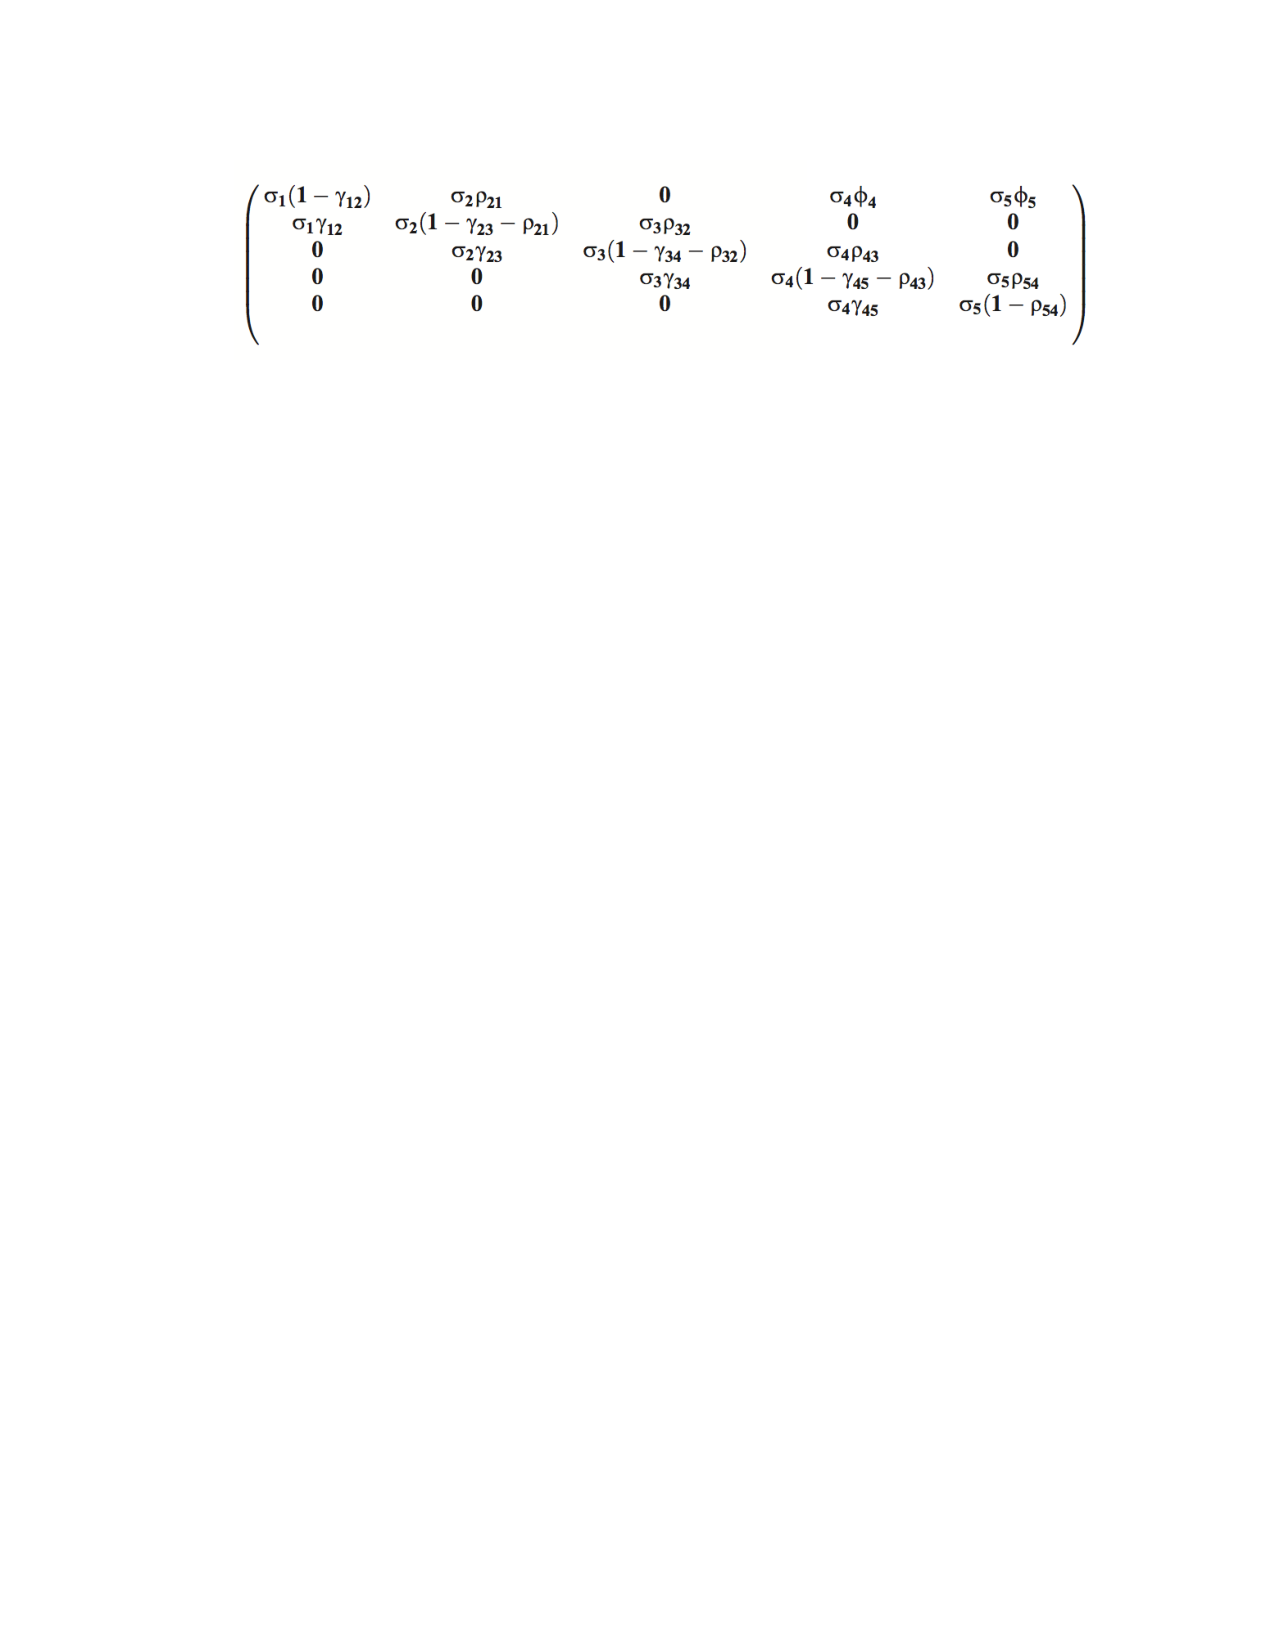
\includegraphics[height=3cm, width=12cm]{Khaya_matrix_model.pdf} \hspace*{2cm}
\end{center}
\begin{itemize}
\item<1> $\sigma_{i}$: survival probabilities \\
\item<1>$\gamma_{ij}$: probability of transitioning from class $i$ to class $j$ \\
\item<1>$\phi_{i}$: fertility rate of adult class \\
\item<1> 6 populations in dry region: 3 high harvest, 3 low harvest; \\
6 populations in moist region: 3 high harvest, 3 low harvest 
\end{itemize}
\end{frame}

\begin{frame}
\frametitle{Previous Work}
\begin{itemize}
\item {\color{beamer@headercolor}  \text{Main results}}: 
\vspace{.1cm}
\begin{enumerate}[-]
\item Effect of NTFP harvest was greater in the short term on population growth rate than the long term, especially in moist region; using long-term growth rates only to inform management decisions for sustainable harvest in the short term can be misleading. 

\item Survival of early, non-reproductive stages is more important for short-term dynamics than long-term dynamics (management decisions made short-term). 
\item  Information on both short and long-term population dynamics should be used for management plans. 
\end{enumerate}
\end{itemize}
\vspace{-.2cm}
\begin{itemize}
\item<1> Generalized harvest of adults as high or low to explore short and long term population growth rates; not explicit with amount of harvest for each size class and harvest did not vary over time.
\item Model did not incorporate the non-lethal harvest of juveniles or lethal harvest of adults.
\item Provides motivation for the development of our model. 

\end{itemize}
\end{frame}

\section{Harvesting Model Formulation}

\begin{frame}
\frametitle{Harvesting Model Formulation}
\begin{itemize}
\item {\color{beamer@headercolor}  \textbf{Goals}}: 
\vspace{.2cm}
\begin{enumerate}[-]
\item Develop a size-dependent, time-varying harvesting model for \textit{K. senegalensis}. 
\vspace{.2cm}
\item Investigate optimal size-dependent harvesting strategies for \textit{K. senegalensis} with the goal of maximizing benefits to the local population, while minimizing the cost of harvesting. 
\end{enumerate}
\end{itemize}
\end{frame}

\begin{frame}
\frametitle{Harvesting Model Formulation}
{\color{beamer@headercolor}  \textbf{Preliminary idea: Continuous model}}
\vspace{.5cm}
\begin{itemize}
\item {\color{beamer@headercolor}  \text{Population Classes}}
\begin{enumerate}[-]
\item Seedlings (S) %0 cm $<$ basal diameter $<$ 5 cm
\item Juveniles (J)  %5 cm $\leq$ diameter at breast height $<$ 20 cm
\item Adults (A) %diameter at breast height $\geq$ 20 cm
\end{enumerate}
\item {\color{beamer@headercolor}  \text{Assumptions}}
\begin{enumerate}[-]
\item Seedlings do not reproduce nor are harvested. 
\item Juveniles do not reproduce and are non-lethally harvested. 
\item Adults reproduce and are both non-lethally and lethally harvested. 
\end{enumerate}
\end{itemize}
\end{frame}


\begin{frame}
\frametitle{Harvesting Model Formulation}
\hspace*{-0.8cm} \includegraphics[height=4cm, width=12cm]{Harvesting_schematic.pdf}\hspace*{1.2cm} 
\begin{center}
Schematic diagram for harvesting model
\end{center}
\end{frame}



\begin{frame}{System of ODEs Model}

\small

$$\dfrac{dS}{dt} = (r_{e}-\alpha_{1} h_{N}-\beta_{1} h_{L})A - (\epsilon-\alpha_{2} h_{N} -\beta_{2} h_{L})S - \mu_{1} S \hspace{1cm} $$ 


\vspace{.1cm}

$$\dfrac{dJ}{dt} = (\epsilon-\alpha_{2} h_{N} -\beta_{2} h_{L}) S -(\eta - \gamma h_{J}) J - \mu_{2} J  \hspace{1cm}$$

\vspace{.1cm}

$$\dfrac{dA}{dt} = (\eta - \gamma h_{J}) J  - h_{L} A -\mu_{3} A, $$ \\
\vspace{1cm} 

$h_{L}$: function of time representing lethal harvest of adults \\
$h_{N}$: function of time representing nonlethal harvest of adults \\
$h_{J}$: function of time representing nonlethal harvest of juveniles \\
Assume $(r_e-\alpha_1 h_{N}-\beta_1 h_{L})$, $(\epsilon-\alpha_{2} h_{N} -\beta_{2} h_{L})$ and $(\eta - \gamma h_{J})$ all $>$ 0.



\end{frame}






\begin{frame}
\frametitle{Harvesting Model Formulation}
\begin{columns}
\begin{column}{0.6\textwidth} 
\small

$$\dfrac{dS}{dt} = (r_{e}-\alpha_{1} h_{N}-\beta_{1} h_{L})A - (\epsilon-\alpha_{2} h_{N} -\beta_{2} h_{L})S - \mu_{1} S \hspace{1cm} $$ 


\vspace{.1cm}

$$\dfrac{dJ}{dt} = (\epsilon-\alpha_{2} h_{N} -\beta_{2} h_{L}) S -(\eta - \gamma h_{J}) J - \mu_{2} J  \hspace{1cm}$$

\vspace{.1cm}

$$\dfrac{dA}{dt} = (\eta - \gamma h_{J}) J  - h_{L} A -\mu_{3} A  $$ \\
\vspace{1cm} 
\end{column}
\begin{column}{0.4\textwidth}
\begin{itemize}
\vspace{-1.1cm} 
\item<1>Parameters:
\begin{enumerate}[-]
\item<1>$r_{e}A$: maximum rate A produce S with no harvest
\item<1> $\alpha_{1} h_N A$: rate A nonlethal harvest reduces S production
\item<1> $\beta_{1} h_L A$: rate A lethal harvest reduces S production
\item<1>  $\epsilon S$: rate S transition to J  
\end{enumerate}
\end{itemize}
\end{column}
\end{columns}
\end{frame}



\begin{frame}
\frametitle{Harvesting Model Formulation}
\begin{columns}
\begin{column}{0.6\textwidth} 
\small

$$\dfrac{dS}{dt} = (r_{e}-\alpha_{1} h_{N}-\beta_{1} h_{L})A - (\epsilon-\alpha_{2} h_{N} -\beta_{2} h_{L})S - \mu_{1} S \hspace{1cm} $$ 


\vspace{.1cm}

$$\dfrac{dJ}{dt} = (\epsilon-\alpha_{2} h_{N} -\beta_{2} h_{L}) S -(\eta - \gamma h_{J}) J - \mu_{2} J  \hspace{1cm}$$

\vspace{.1cm}

$$\dfrac{dA}{dt} = (\eta - \gamma h_{J}) J  - h_{L} A -\mu_{3} A $$ \\
\vspace{1cm} 
\end{column}
\begin{column}{0.4\textwidth}
\begin{itemize}
\vspace{-1.1cm} 
\item<1>Parameters:
\begin{enumerate}[-]
\item<1>$\alpha_{2} h_N S$: rate A nonlethal harvesting delays transition rate of S to J
\item<1> $\beta_{2} h_L S$: rate A lethal harvesting delays the transition rate of S to J
\item<1> $\mu_1 S$: natural mortality rate of S  
\item<1>  $\eta J$: rate J transition to A
\end{enumerate}
\end{itemize}
\end{column}
\end{columns}
\end{frame}




\begin{frame}
\frametitle{Harvesting Model Formulation}
\begin{columns}
\begin{column}{0.6\textwidth} 
\small

$$\dfrac{dS}{dt} = (r_{e}-\alpha_{1} h_{N}-\beta_{1} h_{L})A - (\epsilon-\alpha_{2} h_{N} -\beta_{2} h_{L})S - \mu_{1} S \hspace{1cm} $$ 


\vspace{.1cm}

$$\dfrac{dJ}{dt} = (\epsilon-\alpha_{2} h_{N} -\beta_{2} h_{L}) S -(\eta - \gamma h_{J}) J - \mu_{2} J  \hspace{1cm}$$

\vspace{.1cm}

$$\dfrac{dA}{dt} = (\eta - \gamma h_{J}) J  - h_{L} A -\mu_{3} A $$ \\
\vspace{1cm} 
\end{column}
\begin{column}{0.4\textwidth}
\begin{itemize}
\vspace{-1.1cm} 
\item<1>Parameters:
\begin{enumerate}[-]
\item<1>$\gamma h_J J$: rate J nonlethal harvesting reduces J growth and delays the transition rate of J to A
\item<1>$\mu_2 J$: natural mortality rate of J
\item<1>  $\mu_3 A$: natural mortality rate of A
\end{enumerate}
\end{itemize}
\end{column}
\end{columns}
\end{frame}

\begin{comment}
\begin{frame}
\frametitle{Harvesting Model Formulation}
{\color{beamer@headercolor}  \textbf{Idea 2: Discrete model}}
\vspace{.5cm}
\begin{itemize}
\item {\color{beamer@headercolor}  \text{Population Classes}}
\begin{enumerate}[-]
\item Seedlings (SDL): 0 cm $<$ basal diameter $<$ 2 cm
\item Saplings (SAP):  2 cm $\leq$ basal diameter $<$ 5 cm
\item Juveniles (JUV): 5 cm $\leq$ diameter at breast height $<$ 20 cm
\item Adults (AD): diameter at breast height $\geq$ 20 cm
\end{enumerate}
\item {\color{beamer@headercolor}  \text{Assumptions}}
\begin{enumerate}[-]
\item Seedlings, Saplings do not reproduce nor are harvested. 
\item Juveniles do not reproduce and are non-lethally harvested. 
\item Adults reproduce and are both non-lethally and lethally harvested. 
\end{enumerate}
\end{itemize}
\end{frame}
\end{comment}


\begin{comment}
\begin{frame}{Stage-structured Model}

\small

$$(SDL)_{k+1} = (\sigma_{1} - \alpha_{1} h_{N}- \alpha_{2} h_{L})(1-\gamma_{12})(SDL)_{k} +\sigma_{4}(\phi_{4}-\alpha_{7} h_{N}-\alpha_{8} h_{L})(AD)_{k}  $$

$$(SAP)_{k+1} = (\sigma_{1} - \alpha_{1} h_{N}- \alpha_{2} h_{L})\gamma_{12} (SDL)_{k}+ (\sigma_{2}-\alpha_{3} h_{N } - \alpha_{4} h_{L})(1-\gamma_{23})(SAP)_{k} $$

$$ (JUV)_{k+1} = (\sigma_{2}-\alpha_{3} h_{N} - \alpha_{4} h_{L})\gamma_{23} (SAP)_{k}+ (\sigma_{3}-\alpha_{5}h_{J}) (1-\gamma_{34})(JUV)_{k} $$ \\

$$(AD)_{k+1} = (\sigma_{3}-\alpha_{5}h_{J})\gamma_{34} (JUV)_{k}+ \sigma_{4}(1-h_{L})(AD)_{k} $$ 

\end{frame}
\end{comment}


\begin{comment}
\begin{frame}
\frametitle{Harvesting Model Formulation}
\begin{columns}
\begin{column}{0.7\textwidth} 
\scriptsize

$$(SDL)_{k+1} = (\sigma_{1} - \alpha_{1} h_{N}- \alpha_{2} h_{L})(1-\gamma_{12})(SDL)_{k} +\sigma_{4}(\phi_{4}-\alpha_{7} h_{N}-\alpha_{8} h_{L})(AD)_{k}  $$

$$(SAP)_{k+1} = (\sigma_{1} - \alpha_{1} h_{N}- \alpha_{2} h_{L})\gamma_{12} (SDL)_{k}+ (\sigma_{2}-\alpha_{3} h_{N } - \alpha_{4} h_{L})(1-\gamma_{23})(SAP)_{k} $$

$$ (JUV)_{k+1} = (\sigma_{2}-\alpha_{3} h_{N} - \alpha_{4} h_{L})\gamma_{23} (SAP)_{k}+ (\sigma_{3}-\alpha_{5}h_{J}) (1-\gamma_{34})(JUV)_{k} $$ \\

$$(AD)_{k+1} = (\sigma_{3}-\alpha_{5}h_{J})\gamma_{34} (JUV)_{k}+ \sigma_{4}(1-h_{L})(AD)_{k} $$ \vspace{1cm} 
\end{column}
\begin{column}{0.3\textwidth}
\begin{itemize}
\vspace{-1.2cm} 
\item<1>Parameters:
\begin{enumerate}[-]
\item<1>$\sigma_{i}$: survival probabilities \\
\item<1>$\gamma_{ij}$: probability of transitioning from class $i$ to class $j$ \\
\item<1>$\phi_{i}$: fertility rate of adult class \\
\end{enumerate}
\end{itemize}
\end{column}
\end{columns}
\end{frame}
\end{comment}



\begin{frame}
\frametitle{Future Tasks}
\begin{itemize}
\item<1> Further develop a harvesting model and analyze (currently deciding between continuous and discrete). 
\vspace{0.5cm}
\item<1> Determine best size-dependent harvesting strategies for \textit{K. senegalensis} to maximize benefits of harvest and conservation of the species, while minimizing harvesting costs. 

\end{itemize}
\end{frame}



\begin{frame}
\frametitle{Units}
Heroin Model:
\begin{itemize}
\item<1> $S, P, A, H, R$: unit-less because proportions 
\item<1> $t$: year
\item<1> $\xi$: unit-less
\item<1> All other parameters: 1/year 
\end{itemize} 

\vspace{0.5cm}

Harvesting Model:
\begin{itemize}
\item<1> $S, J, A$: number of trees
\item<1> $t$: year
\item<1> $\alpha_1, \alpha_2, \beta_1, \beta_2, \gamma$: unit-less
\item<1> $h_N, h_L$: 1/year
\item<1> All other parameters: 1/year
\end{itemize}

\end{frame}




%\begin{comment}

\begin{frame}
\frametitle{References}
\begin{enumerate}[-]
\scriptsize
\item Bufford, J. L. and Gaoue, O. G. (2015), Defoliation by pastoralists affects savanna tree seedling dynamics by limiting the facilitative role of canopy cover. Ecological Applications, 25: 1319-1329. doi:10.1890/14-0953.1 
\item Driessche, P. van den, and James Watmough. "Further Notes on the Basic Reproduction Number." SpringerLink, Springer, Dordrecht, 1 Jan. 1970, link.springer.com/chapter/10.1007/978-3-540-78911-6$_$6
\item Gaoue, O. G., Ngonghala, C. N., Jiang, J. and Lelu, M. (2016), Towards a mechanistic understanding of the synergistic effects of harvesting timber and non-timber forest products. Methods Ecol Evol, 7: 398-406. 
\item Gaoue, O. G., Jiang, J., Ding, W., Agusto, F. B., & Lenhart, S. (2016). Optimal harvesting strategies for timber and non-timber forest products in tropical ecosystems. Theoretical Ecology, 9(3), 287-297. doi:http://dx.doi.org/10.1007/s12080-015-0286-4
\item Gaoue, O. G. (2016), Transient dynamics reveal the importance of early life survival to the response of a tropical tree to harvest. J Appl Ecol, 53: 112-119. doi:10.1111/1365-2664.12553
\item  Gaoue OG (2015) Data from: Transient dynamics reveal the importance of early life survival to the response of a tropical tree to harvest. Dryad Digital Repository. https://doi.org/10.5061/dryad.mb1d0




\end{enumerate}
\end{frame}

%\end{comment}


%\begin{comment}
\begin{frame}
\frametitle{References}
\begin{enumerate}[-]
\scriptsize 
\item Han B, Compton WM, Blanco C, Crane E, Lee J, Jones CM. (2017), Prescription Opioid Use, Misuse, and Use Disorders in U.S. Adults: 2015 National Survey on Drug Use and Health. Ann Intern Med,167:293-301. doi: 10.7326/M17-0865
\item Hughs, Arthur, et al. Prescription Drug Use and Misuse in the United States: Results from the 2015 National Survey on Drug Use and Health. Sept. 2016, www.samhsa.gov/data/sites/default/files/NSDUH-FFR2-2015/NSDUH-FFR2-2015.htm
\item Key Substance Use and Mental Health Indicators in the United States: Results from the 2015 National Survey on Drug Use and Health. www.samhsa.gov/data/sites/default/files/NSDUH-FFR1-2015/NSDUH-FFR1-2015/NSDUH-FFR1-2015.pdf
\item Key Substance Use and Mental Health Indicators in the United States: Results from the 2016 National Survey on Drug Use and Health. www.samhsa.gov/data/sites/default/files/NSDUH-FFR1-2016/NSDUH-FFR1-2016.pdf
\item Mandell, Brian F. The Fifth Vital Sign: A Complex Story of Politics and Patient Care. June 2016, www.mdedge.com/sites/default/files/issues/articles/Mandell$_$June16$_$Blurb.pdf.
\item Medication-Assisted Treatment. www.samhsa.gov/medication-assisted-treatment
\item Muhuri, Pradip K., et al. Associations of Nonmedical Pain Reliever Use and Initiation of Heroin Use in the United States. Aug. 2013, archive.samhsa.gov/data/2k13/DataReview/DR006/nonmedical-pain-reliever-use-2013.pdf.
\end{enumerate}
\end{frame}

%\end{comment}


%\begin{comment}

\begin{frame}
\frametitle{References}
\begin{enumerate}[-]
\scriptsize 
\item National Institute on Drug Abuse (NIDA) Prescription Opioids and Heroin. d14rmgtrwzf5a.cloudfront.net/sites/default/files/19774-prescription-opioids-and-heroin.pdf
\item Opioid Overdose. Centers for Disease Control and Prevention, Centers for Disease Control and Prevention, 16 Dec. 2016, www.cdc.gov/drugoverdose/data/fentanyl.html
\item Potter, J. S., Marino, E. N., Hillhouse, M. P., Nielsen, S., Wiest, K., Canamar, C. P., ... Ling, W. (2013). Buprenorphine/naloxone and methadone maintenance treatment outcomes for opioid analgesic, heroin, and combined users: Findings from starting treatment with agonist replacement therapies (START). Journal of Studies on Alcohol and Drugs, 74(4), 605-613
\item Results from the 2016 National Survey on Drug Use and Health. www.samhsa.gov/sites/default/files/sites/default/files/2016$_$ffr$_$1$_$slideshow$_$v5.pdf
\item U.S. and World Population Clock. www.census.gov/popclock/
\item Volkow, Nora D. ``America's Addiction to Opioids: Heroin and Prescription Drug Abuse.'' NIDA, 14 May 2014, www.drugabuse.gov/about-nida/legislative-activities/testimony-to-congress/2016/americas-addiction-to-opioids-heroin-prescription-drug-abuse$#_$ftn2
\item 2016 NSDUH Report: America{'}s Behavioral Health Changes and Challenges. www.samhsa.gov/sites/default/files/topics/data$_$outcomes$_$quality/nsduh-ppt-09-2017.pdf 

\end{enumerate}
\end{frame}

%\end{comment}


\end{document}